\chapter[Solução de Energia]{Solução de Energia}
\label{Solução_energia}

% Cada frente deve adc os subtópicos que acharem pertinentes

O escopo da solução energética do projeto envolve a implementação de uma fonte de alimentação principal, uma fonte de alimentação alternativa e um sistema eletromecânico. Todos esses componentes serão ocultados do campo de visão do usuário. Os objetivos da solução envolvem alcançar um custo reduzido, alta eficiência, robustez e compactação da estrutura. A configuração da solução da alimentação do sistema está representada no diagrama de blocos simplificado da Fig. \ref{fig:energia_alimentacao}.

\begin{figure}[H]
    \centering
    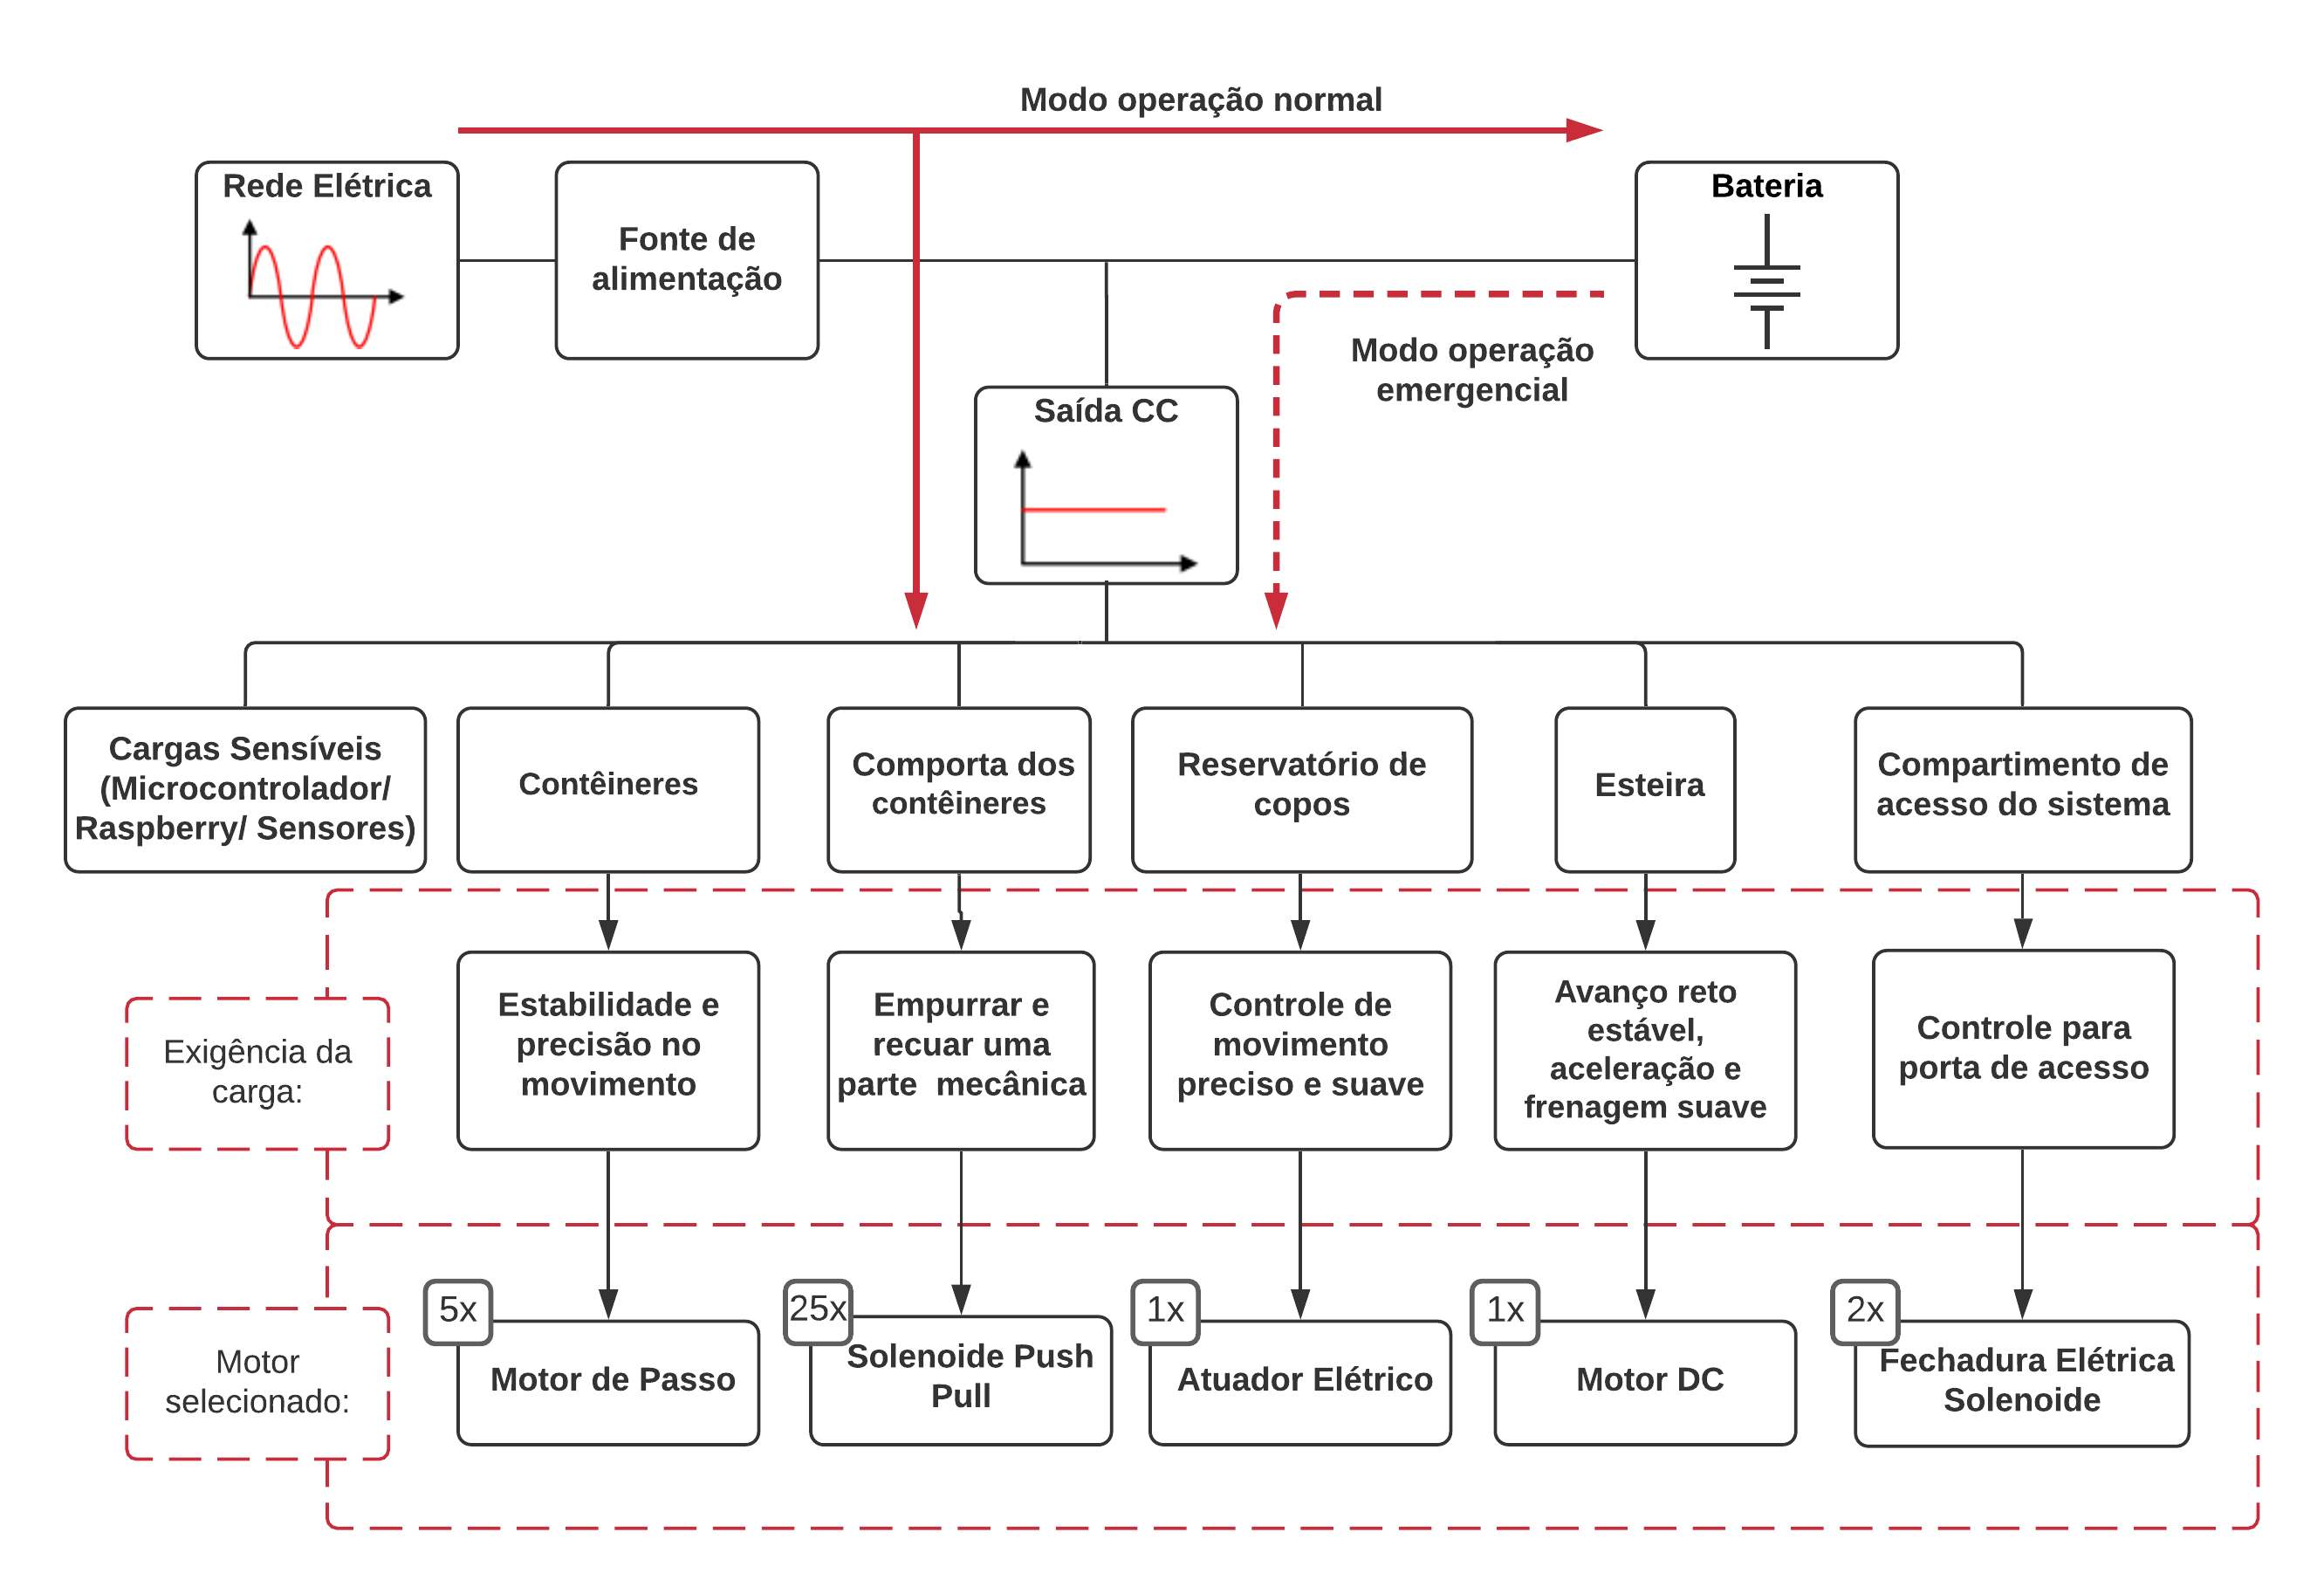
\includegraphics[width=1\textwidth]{figuras/energia/esq_alimentacao.png}
    \caption{Esquema do sistema de alimentação proposto.}
    \label{fig:energia_alimentacao}
\end{figure}

A carga do projeto será atendida de duas maneiras, considerando dois modos de operação: pela fonte de alimentação, quando houver energia elétrica na rede, e por uma fonte de alimentação alternativa, cuja função será atuar como uma fonte auxiliar/secundária que assegurará a ininterruptibilidade no provimento de energia, em casos de falha da energia proveniente da rede primária.

\section{Sistema eletromecânico}

A escolha dos motores é baseada nas características técnicas das aplicações, nas exigências das cargas e na alimentação do sistema no que se refere ao ponto de vista mecânico para avaliar o conjugado de aceleração, de partida e o nominal \cite{santos_2016}. Essas características serão comparadas com as características dos motores, para a seleção adequada dos mesmos. Os seguintes itens foram considerados:

\begin{enumerate}
    \item[ ]
    \begin{itemize}
        \item[ ]
        \begin{itemize}
            \item Redução de custos;
            \item Conjugados solicitados;
            \item Dispensabilidade ou não de regulação de velocidade;
            \item Menor espaço ocupado (horizontal e vertical);
            \item Rendimento;
           % \item Aumento de temperatura;
            \item Funcionalidade e viabilidade (benefício pelo ônus);
            \item Segurança;
          %  \item Menor exigência de potência (economia de energia).
          %  \item Menor índice de falhas;
          %  \item Facilidade de manutenção;
            \item Versatilidade do controle dinâmico.
        \end{itemize}
    \end{itemize}
\end{enumerate}

O dimensionamento e a seleção adequados de um motor para um equipamento são essenciais para garantir a confiabilidade, o desempenho e o custo do equipamento. Logo, os motores foram selecionados, com base nas especificações requeridas. Após essa seleção, foi feita uma determinação final do motor, confirmando que as especificações dos motores selecionados satisfazem todos os requisitos.

%O primeiro passo para dimensionar um motor elétrico é determinar certas características do projeto, como o mecanismo de acionamento, dimensões aproximadas, distâncias percorridas e período de posicionamento.

%Junto com o tipo de mecanismo de acionamento, também será necessário determinar as dimensões, massa e coeficiente de atrito que são necessários para o cálculo de carga:

%\begin{enumerate}
 %   \item[ ]
%    \begin{itemize}
    %    \item[ ]
   %     \begin{itemize}
  %          \item Dimensões e massa (ou densidade) da carga;
 %           \item Dimensões e massa (ou densidade) de cada parte;
%            \item Coeficiente de atrito da superfície deslizante de cada peça %móvel;
  %      \end{itemize}
 %   \end{itemize}
%\end{enumerate}

%Em seguida, foi preciso designar as especificações necessárias para o equipamento:

%\begin{enumerate}
%    \item[ ]
 %   \begin{itemize}
  %      \item[ ]
   %     \begin{itemize}
    %        \item Velocidade operacional e tempo operacional;
     %       \item Distância de posicionamento e tempo de posicionamento;
      %      \item Precisão de parada;
       %%%%% \item Ambiente operacional. %(Caixa fechada, Temperatura mínima X, Temperatura Máxima Y).
      %  \end{itemize}
    %\end{itemize}
%\end{enumerate}


%Após todas as definições acima, é fundamental determinar o desempenho do motor, calculando o movimento de inércia, o torque e velocidade no eixo de acionamento.

%MOVIMENTO DE INÉRCIA: FÓRMULA
%TORQUE : FÓRMULA
%VELOCIDADE: FÓRMULA

\subsection{Motor de passo}\label{sec:energia_motor_passo}

 O dispositivo eletromecânico responsável pelo deslocamento e disposição dos compartimentos que armazenam os medicamentos será um motor de passo de corrente contínua. Ele é capaz de suprir o torque requerido pelo fuso que irá rotacionar a base dos compartimentos, permitindo a orientação dos comprimidos à saída. A escolha desse motor se deu pela sua capacidade de produzir alto torque em baixa velocidade e, ao mesmo tempo, minimizar a vibração. Seu dimensionamento levou em consideração os seguintes itens: 

\begin{itemize}
    \item Torque dos contêineres: 0,16 N$\cdot$m, calculado por meio da Eq. \ref{energia_torque_cont}, onde a inércia (I), calculado no software \textit{Catia} tem o valor de 1,857 $10^-5$ kg$\cdot$m$^2$, e o $\alpha $ um valor de $\pi${$rad$}/{$s^2$},calculado por meio da Eq. \ref{energia_torque_alpha}.

    \begin{equation}
        \tau = I \cdot \alpha
        \label{energia_torque_cont}
    \end{equation}
    %\left(  \right)

        \begin{equation}
        \alpha = \theta_{o} + \frac{1}{2} \cdot (w_{f} + w_{o}) \cdot t
        \label{energia_torque_alpha}
    \end{equation}
    %\left(  \right)
    
    Onde, $\theta_{o}$ e $w_{o}$ são iguais a zero, o tempo ($t$) é 1 segundo e $w_f$ é 2$\pi$ rad/s.
   
   % \item Potência do motor de passo: 4,8 W, calculaca por meio da equação .

    %\item Velocidade angular: estimada como sendo igual a 1/60 rpm; %pq?
    
\end{itemize}

 \begin{figure}[H]
\centering
    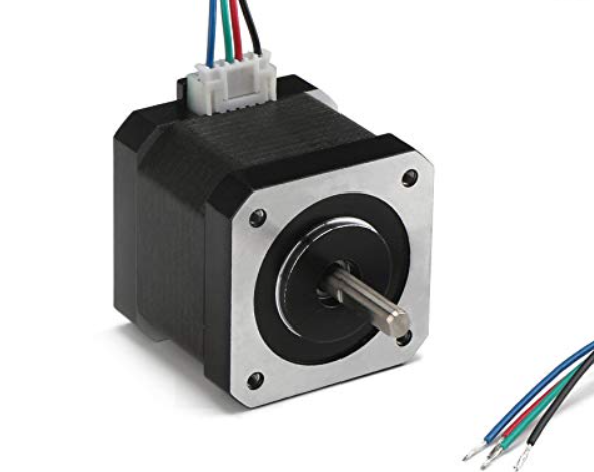
\includegraphics[width=0.35\textwidth]{figuras/energia/fotos_componentes/Energia_passo.png}
    \caption{Motor de Passo 42HS40-0404.}
    \label{fig:energia_passo}
\end{figure}


 Com base nesses dados, optou-se pela escolha do motor de passo padrão Nema17 - KTC-42HS40-0404, da marca Kalatec Automação, representado na Fig. \ref{fig:energia_passo}, pois suas especificações técnicas atendem aos requisitos do projeto. Este motor apresenta um torque nominal 0,40 N$\cdot$m e potência de 4,8 W . O motor apresenta um controle preciso de posição, torque e velocidade, que são fatores necessários para fazer rotacionar o fuso, dando torque às engrenagens dos contêineres, que distribuirão os comprimidos.
 
 
 \subsection{Motor DC}\label{energ:motor_dc}

No plano inferior do projeto, onde temos o repositório de copos, também há uma esteira de locomoção que tem, por objetivo, efetuar a locomoção dos copos com os medicamentos até a saída do produto. Esta será acionada por meio de um motor DC de eixo simples. A escolha desse dispositivo se deu ao considerar um menor custo, boa economia de energia e fácil operação. Seu dimensionamento levou em consideração os seguintes itens:

\begin{itemize}
    \item Torque do motor DC: 1,8 N$\cdot$m, calculado por meio da Eq. \ref{energia_torque_dc}, onde o raio (r) é 61,05 mm, a força (F) tem o valor de 30 N e o ângulo theta entre ambos é de $90${$^\circ$}.

    \begin{equation}
        \tau = r \cdot F \cdot seno(\theta)
        \label{energia_torque_dc}
    \end{equation}
    %\left(  \right)
    
    %\item Velocidade nominal: 12 rpm; %pq?
    
    %\item Potência máxima do motor DC: 19,2 W;
    \item Distância que o copo irá percorrer até a saída: 570 mm;
    %\item Inércia: $4,746 \times 10^{-5}$  kg$ \cdot $m$^2$;
     %\item Massa do conjunto: 3 kg; 
\end{itemize}

\begin{figure}[H]
\centering
    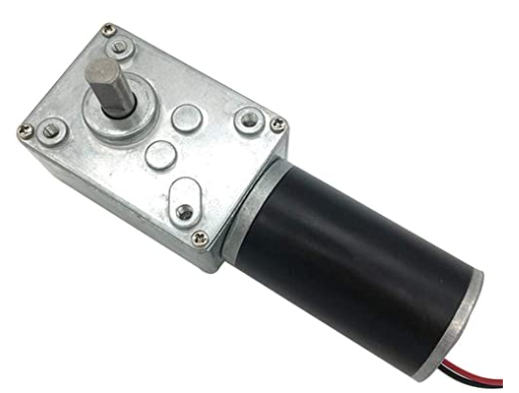
\includegraphics[width=0.35\textwidth]{figuras/energia/fotos_componentes/Energia_dc.png}
    \caption{Motor DC \emph{Bringsmart} 12 V}
    \label{fig:energia_dc}
\end{figure}



Em pesquisa de mercado, optou-se pela escolha do motor \emph{Bringsmart} 12 V, da marca \emph{Hugwit Company}, representado na Fig. \ref{fig:energia_dc}, por suas especificações técnicas atenderem os requisitos do projeto. Este apresenta um torque de 6,8 N$\cdot$m com potência de 19,2 W. 
 
\subsection{Mini Atuador elétrico linear}\label{energ:atuador_linear}

O controle de atuação linear no reservatório de copos será por meio de um mini atuador elétrico linear. O atuador elétrico linear converte movimento rotativo em uma voltagem contínua em movimento linear. A escolha deste dispositivo de acionamento se deu pela facilidade de instalação, operação e velocidade constante. Seu dimensionamento levou em consideração os seguintes itens:

\begin{itemize}
   % \item Força linear necessária para mover o copo = 0,1 N;
    \item Distância linear que o copo precisar percorrer até a esteira: 90 mm;
    \item O tempo requerido para movimentar o copo: 5 s;
\end{itemize}

\begin{figure}[H]
\centering
    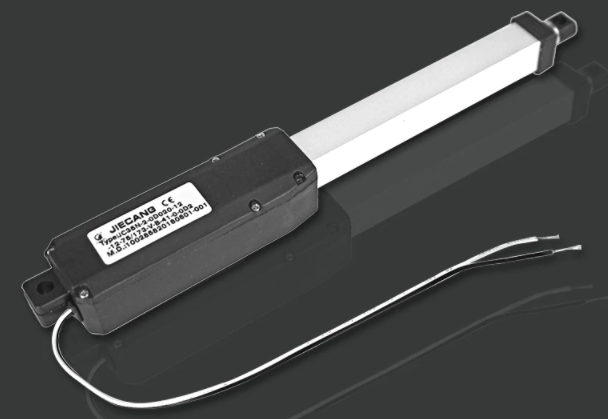
\includegraphics[width=0.5\textwidth]{figuras/energia/fotos_componentes/Energia_atuador.png}
    \caption{Mini-Atuador Elétrico Selecionado}
    \label{fig:energia_atuador}
\end{figure}


Dessa forma, o atuador dimensionado foi o mini atuador elétrico linear, representado na Fig. \ref{fig:energia_atuador}. Este apresenta torque de 20 N, com haste de 100 mm e velocidade constante de 15 mm/s.

\subsection{Solenoide}\label{energ:solenoide}

O dispositivo eletromecânico responsável pela abertura e fechamento das comportas, que liberam os medicamentos para seus canais de guia, será um eletroímã solenoide elétrico - atuador \textit{Push Pull}. Quando acionado, ele irá abrir uma pequena porta, onde só irá descer um comprimido por vez. A escolha desse dispositivo se deu pela facilidade de instalação, operação e movimento linear.
Para a porta de saída do dispositivo, o acionamento se dará por meio de uma fechadura elétrica solenoide, que a sustentará na posição aberta, até que o copo com o medicamento seja entregue ao usuário. Além dessa, também serão utilizadas 6 solenoides na parte superior da carcaça do projeto, nas portas de manutenção dos contêineres, com funcionamento semelhante ao explicitado anteriormente.

\begin{figure}[H]
\centering
\subfloat[][Mini Solenoide Eletro-imã Dc 12v \textit{Push Pull}.]{
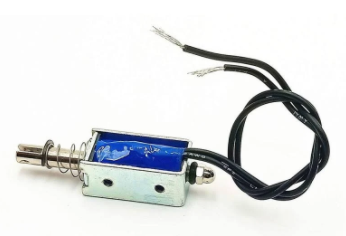
\includegraphics[width=0.4\textwidth]{figuras/energia/fotos_componentes/Energia_push.png}
\label{fig:energia_push}}
\qquad
\subfloat[][Mini Trava Elétrica Solenoide 12V.]{
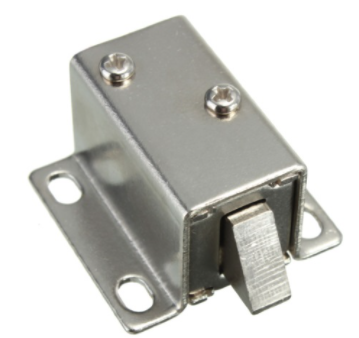
\includegraphics[width=0.3\textwidth]{figuras/energia/fotos_componentes/Energia_porta.png}
\label{fig:energia_porta}}
\caption{Solenoides selecionadas para o projeto.}
%\label{fig:globfig}
\end{figure}

A solenoide selecionada para abertura da porta dos compartimentos é da marca ECSZINX, modelo \textit{Push Pull} 12 V, representada na Fig. \ref{fig:energia_push} e, para o controle da porta de acesso e das portas superiores de manutenção, foi selecionada uma Mini Trava Elétrica Solenóide 12 V, da marca AT, representada na Fig. \ref{fig:energia_porta}.

\section{Fonte de Alimentação Principal} \label{section:energia_fonte}

% Para o fornecimento de energia elétrica necessária ao motor e circuitos eletrônicos do dispensador, 
 
 O dispositivo que converte a energia elétrica disponibilizada pela concessionária para uma tensão, corrente e frequência exigida por algum eletroeletrônico é a fonte de alimentação. Desse modo, a fim de atender as necessidades energéticas do projeto, o dispensador \textit{Pill Watcher} contará com uma fonte de alimentação comutada ou chaveada (\textit{switched-mode power supply} - SMPS), que terá prioridade no sistema de energização do equipamento. Os fatos que motivaram a escolha de desenvolver uma fonte chaveada em relação a uma fonte linear são \cite{Projeto_fonte}:
 
 %MUDAR PARA UMA TABELA COMPARATIVA
 \begin{enumerate}
    \item[ ]
    \begin{itemize}
        \item[ ]
        \begin{itemize}
            \item Menor tamanho;
            \item Menor peso;
            \item Maior eficiência;
            \item Menor geração de calor;
            \item Baixo consumo;
            \item Equipamento mais compacto.
        \end{itemize}
    \end{itemize}
\end{enumerate}

O dimensionamento das duas fontes de alimentação será determinado principalmente pelo sistema embarcado e motores que atendam ao sistema de operação, e levará em conta sua distribuição espacial no equipamento. A Tab. \ref{fig:energia_carga} contém o levantamento da carga do sistema.

%A configuração contará com um sistema de proteção contra curto-circuito, sobrecarga, sobretensão, baixa tensão e ligação inversa da bateria.
 
\begin{table}[htb]
    \centering
    \caption{Levantamento da carga do projeto.}
    \label{fig:energia_carga}
    \begin{adjustbox}{max width = \textwidth}
        \begin{tabular}{|L{5cm}|C{2cm}|C{2cm}|C{2cm}|C{2cm}|C{2cm}|}
            \hline
            \rowcolor[HTML]{A8DADC}
           \multicolumn{1}{|c|}{ \textbf{Equipamento}} & \textbf{Quant. (unid.)} & \textbf{Tensão (unid.) [V]} & \textbf{Corrente (unid.) [A]} & \textbf{Potência (total) [W]} \\ \hline
            Sensor de Temperatura e Umidade & 1	 & 3,3 & 0,05x10E-2 & 0,15x10E-2
            \\ \hline
           %   Sensor Fotoelétrico Emissor & 30	 & 3,3 & 0,1 & 9,9
         %   \\ \hline
              Sensor Fotoelétrico & 30	 & 5  & 0,25x10E-1 & 3,75
             \\ \hline
             Sensor de Biometria & 1 & 5 & 0,12 & 0,6
             \\ \hline
             Sensor de Leitor RFID & 1	 & 5 & 0,25x10E-1 & 1,25x10E-1
             \\ \hline
              \textit{Raspberry Pi} 4 & 1 & 5 & 3 & 15
             \\ \hline
               Microcontrolador & 4 & 5 & 0,25x10E-1 & 0,5
             \\ \hline
               Visor & 1 & 5 & 0,02 & 0,1
             \\ \hline
               Câmera & 1 & 3,3 & 0,2 & 0,66
             \\ \hline
            %  Teclado & 1 & X & X & X
            % \\ \hline
            %  Cls Mux/Demux & 12 & 5 & 0,000001 & 
            % \\ \hline
              Fechadura Elétrica Solenoide & 7 & 12 & 0,5 & 42
             \\ \hline
              Motor de Passo & 5 & 12 & 0,4 & 24
             \\ \hline
              Eletroímã Solenoide elétrico - atuador \textit{Push Pull} & 25 & 5 & 1,12 & 140
             \\ \hline
                Motor DC & 1 & 12 & 1,6 & 19,2
             \\ \hline
                Atuador Linear Elétrico & 1 & 12 & 2 & 24
             \\ \hline
               \textit{Driver} A4988 & 5 & 12 & 0,5 & 30
             \\ \hline
                \textit{Driver} IRF520N & 33 & 12 & 2 & 792
             \\ \hline
                  \textit{Driver} L298N & 1 & 12 & 1,6 & 19,2
             \\ \hline
             \rowcolor[HTML]{F1FAEE}
             \multicolumn{4}{|l|}{\cellcolor[HTML]{F1FAEE}Total} & 1157,14 \\
             \hline
        \end{tabular}
    \end{adjustbox}
\end{table}

A potência instalada do equipamento é igual a 1157,14 W. A fonte de alimentação e a fonte auxiliar deverão ser dimensionadas com base na corrente total e no potencial de falha do pior caso. O diagrama unifilar do projeto encontra-se na Fig. \ref{fig:diagrama_fonte1}. Portanto, serão considerados os seguintes cenários representados na Tab. \ref{fig:energia_cenarios}. 

Para o cenário 1, todas as cargas são acionadas ao mesmo tempo, o que é improvável de acontecer, pois a premissa do funcionamento do equipamento é que só um medicamento pode ser expelido por vez. No cenário 2, é considerado que seriam acionados ao mesmo tempo um motor de passo, uma solenoide, o atuador e as travas elétricas. 

\begin{table}[H]
    \centering
    \caption{Cenários considerados para o dimensionamento dos sistemas de alimentação.}
    \label{fig:energia_cenarios}
    \begin{adjustbox}{max width = \textwidth}
        \begin{tabular}{|L{5cm}|C{2cm}|C{2cm}|C{2cm}|C{2cm}|C{2cm}|}
            \hline
            \rowcolor[HTML]{A8DADC}
           \multicolumn{1}{|c|}{ \textbf{Equipamento}} & \textbf{Cenário 1} & \textbf{Cenário 2} & \textbf{Cenário 3} & \textbf{Cenário 4} \\ \hline
            Sensor de Temperatura e Umidade & x1 & x1 & x1 & x1
            \\ \hline
           %   Sensor Fotoelétrico Emissor & 30	 & 3,3 & 0,1 & 9,9
         %   \\ \hline
              Sensor Fotoelétrico & x30	 & x30 & x30 & x30
             \\ \hline
             Sensor de Biometria &  x1	 & x1 & x1 & x1
             \\ \hline
             Sensor de Leitor RFID & x1	 & x1  & x1 & x1
             \\ \hline
             \textit{Raspberry Pi} 4 & x1 & x1 & x1 & x1
             \\ \hline
               Microcontrolador & x4 & x4 & x3 & x4
             \\ \hline
               Visor & x1	 & x1 & x1 & x1
             \\ \hline
               Câmera & x1 & x1 & x1 & x1
             \\ \hline
            %  Teclado & 1 & X & X & X
            % \\ \hline
            %  Cls Mux/Demux & 12 & 5 & 0,000001 & 
            % \\ \hline
              Fechadura Elétrica & x2	 & x2 & - & -
             \\ \hline
              Motor de Passo & x5 & x1 & x1 & x1
             \\ \hline
             Atuador \textit{Push Pull} & x25	 & x1 & - & -
             \\ \hline
                Motor DC & x1 & x1 & x1 & -
             \\ \hline
                 Atuador Linear Elétrico & x1 & x1 & - & x1
             \\ \hline
               \text{Driver} para Motor de Passo & x5 & x1 & x1 & x1
             \\ \hline
                \textit{Driver} IRF 520 & x33 & x1 & - & x1
             \\ \hline
                  \textit{Driver} Ponte H & x1 & x1 & x1 & -
             \\ \hline
             \rowcolor[HTML]{F1FAEE}
             \multicolumn{1}{|l|}{\cellcolor[HTML]{F1FAEE}Corrente Total (A) } & x & 13,82 & 8,29 & 9,12 \\
             \hline
        \end{tabular}
    \end{adjustbox}
\end{table}

Para os cenários 3 e 4 são considerados as seguintes premissas: 
    
    \begin{itemize}
        
        \item O medicamento não pode ser liberado da comporta enquanto o contêiner estiver em movimento, ou seja, o motor de passo e a solenoide não podem ser acionados ao mesmo tempo;
        
        \item Não será possível colocar um copo na esteira em movimento, ou seja, o atuador elétrico e o motor DC não podem ser acionados ao mesmo tempo;
        
        \item Não será possível liberar um medicamento enquanto a esteira estiver em movimento, ou seja, a solenoide, o motor DC e o atuador elétrico não podem ser acionados ao mesmo tempo;
        
        \item O contêiner pode estar em movimento enquanto um copo com medicamento está sendo levado para a saída do equipamento, ou seja, o motor de passo e o motor DC podem ser acionados ao mesmo tempo;
        
        \item O contêiner pode estar em movimento enquanto um copo é colocado na esteira, ou seja, o motor de passo e o atuador elétrico podem ser acionados ao mesmo tempo;
        
        \item O contêiner pode estar em movimento enquanto a porta de saída do remédio é aberta, ou seja, o motor de passo e a trava elétrica podem ser acionados ao mesmo tempo;

    \end{itemize}

Com base nas premissas apresentadas acima, considerou-se no cenário 3 onde um motor de passo e o motor DC estariam funcionando ao mesmo tempo. Já no cenário 4, é considerado que um motor de passo e o atuador elétrico funcionariam ao mesmo tempo.

Ao avaliar os cenários propostos percebe-se que, para o dimensionamento dos sistemas de alimentação, os cenários 3 e 4 são os mais apropriados, pois satisfazem às premissas levantadas para o bom funcionamento do equipamento. Portanto, a maior corrente entre os dois cenários será selecionada, e, por cima deste valor, será considerado um fator de segurança igual a 1,7, o que nos leva a uma corrente de projeto aproximadamente igual a 15 A.

Dessa forma, a fonte de alimentação proposta será interligada à rede e proverá uma saída CC regulada igual a 12 V e 15 A de saída, portanto, terá uma potência de 180 W. As cargas que exigirem uma tensão específica contarão com um regulador de tensão. Como os componentes eletrônicos não demandam corrente alternada, a solução não tem a necessidade de englobar um inversor de corrente. As conexões da fonte serão combinadas com o sistema de alimentação alternativo previsto pela bateria. 

\subsection{Retificador CA/CC}
%interface entre a carga e a rede elétrica

%retificadores passivos (não controlados) 
%Retificador ativo com alto fator de potência

Conversores CA/CC, ou retificadores, convertem uma tensão alternada em uma tensão de saída contínua estável. Os retificadores são classificados de acordo com a capacidade de ajuste do valor da tensão de saída (controlados ou não-controlados), o número de fases da tensão de entrada (monofásico, trifásico,etc.) e com os elementos retificadores. Os retificadores não-controlados utilizam diodos como elementos de retificação. O retificador com ponte de onda completa (\textit{full bridge}), topologia mais aplicada em equipamentos na prática, utiliza quatro diodos para converter os ciclos positivos e negativos para o lado CC, antes de estabilizar a tensão de saída com um capacitor \cite{Conversores,Conversores2}. 

Portanto, a etapa de entrada da fonte é baseada em um conversor CC/CC com ponte de onda completa, com sua configuração representada na Fig. \ref{fig:energia_retificador}, onde $L_{ac}$ e $R_{ac}$ são, respectivamente, a indutância e resistência da impedância da fonte alternada de entrada, $D_{1}$, $D_{2}$, $D_{3}$ e $D_{4}$ formam o retificador monofásico de onda completa, e $C_{o}$ é o filtro capacitivo de saída. Seus benefícios e, portanto, a justificativa para a escolha da topologia, são \cite{retificador}:

\begin{itemize}
    \item Em relação aos retificadores de meia onda, possuem maior eficiência de retificação;
    
    \item Possuem baixa perda de energia, pois nenhum sinal de tensão é perdido no processo de conversão;
    
    \item Não necessita de transformador com derivação central;
    
    \item A corrente na carga flui em um único sentido.
\end{itemize}

%\begin{figure}[H]
%\centering
%    \includegraphics[width=0.8\textwidth]{figuras/Energia_Full_bridge.png}
%    \caption{Configuração do retificador com ponte de onda completa a ser implementado com indicação do fluxo de corrente (setas vermelhas). Fonte: \citeonline{Conversores}, com modificações do autor.}
%    \label{fig:energia_retificador}
%\end{figure}

\begin{figure}[H]
\centering
\subfloat[][]{
\includegraphics[width=0.4\textwidth]{figuras/energia/circuitos/Energia_Full_bridge.png}
\label{fig:energia_retificador}}
\qquad
\subfloat[][]{
\includegraphics[width=0.3\textwidth]{figuras/energia/circuitos/retificador_onda.png}
\label{fig:subfig_ondas}}
\caption{Configuração com indicação do fluxo de corrente (setas vermelhas) e formas de onda típicas do retificador de onda completa. Fonte: \citeonline{Conversores}, com modificações do autor.}
\label{fig:globfig}
\end{figure}

A cada meio período da tensão alternada de entrada, há um par de diodos conduzindo. Dessa forma, modelando a carga como sendo resistiva e observando as formas de onda típicas (Fig. \ref{fig:subfig_ondas}), podemos descrever a operação do retificador nas seguintes etapas \cite{retificador}:

\begin{itemize}
    \item  No semiciclo positivo, os diodos $D_{1}$ e $D_{4}$ estão conduzindo, os diodos $D_{2}$ e $D_{3}$ estão bloqueados e o capacitor $C_{o}$ é carregado até o valor máximo da tensão de entrada;
    
    \item A partir do momento que a tensão pulsante é reduzida, ficando menor que a tensão no capacitor, este começa a descarregar, fornecendo energia à carga. Nesta etapa, o capacitor não se descarrega completamente;
    
    \item No semiciclo negativo, os diodos $D_{2}$ e $D_{3}$ estão conduzindo, os diodos $D_{1}$ e $D_{4}$ estão bloqueados e o processo de carregamento do capacitor $C_{o}$ começa novamente. Dessa forma, cerca de metade da energia do capacitor é descarregada e a corrente flui para a carga em uma única direção;
    
\end{itemize}

%\begin{equation}
 % f(x)=\begin{cases}
 %   1, & \text{if $x<0$}.\\
 %   0, & \text{otherwise}.
 % \end{cases}
%\end{equation}

O objetivo da configuração é garantir uma tensão de saída CC constante. A configuração proposta garantirá uma alimentação bivolt, e sua saída é responsável por alimentar a etapa do conversor CC/CC da fonte proposta.

\begin{table}[H]
    \centering
    \footnotesize
    \caption{Parâmetros de projeto do retificador monofásico com ponte de onda completa.}
    \label{retificador}
    \begin{adjustbox}{max width = \textwidth}
        \begin{tabular}{|l|c|c|}
            \hline
            \rowcolor[HTML]{A8DADC}
            \textbf{Parâmetro} & \textbf{Simbologia} & \textbf{Valor}  \\ \hline
            Tensão eficaz de Entrada & $V_{CA}$ & 127/220 [V$_\text{cc}$]
            \\ \hline
           % Tensão máxima de Entrada* & $V_{CAmax}$ & 133/231
            %\\ \hline
            %Tensão mínima de Entrada* & $V_{CAmin}$ & 117/202
           % \\ \hline
              Potência de saída & $P_{o}$	 & 200 [V]
             \\ \hline
              Frequência da Rede & $f_{r}$	 & 60 [Hz]
             \\ \hline
            %  Frequência de Chaveamento & $f_{s}$	 & -Hz
             %\\ \hline
           %     Tensão de Saída & $v_{out}$ & -
            % \\ \hline
            %  Indutor e resistor do \textit{Boost} & L e R & -
            % \\ \hline
           % Impedância da fonte & $ L_{ac}$, $R_{ac}$ &- 
            % \\ \hline
             %   Ondulação da Corrente no Indutor & $\Delta I_{L}$ &- 
            % \\ \hline
               Ondulação da Tensão no Capacitor (\textit{ripple} máximo) & $\Delta V_{C}$ & 10\%
             \\ \hline
                Rendimento & $\eta$ & 0,9
             \\ \hline
            %    fator de ciclo (\textit{duty cycle}) & $D$ & -
             %\\ \hline
            % \multicolumn{3}{l}{*Valores baseados na tabela 4 (Anexo 1)
 %do módulo 8 do Prodist.} \\
              \multicolumn{3}{l}{NOTA: Este design é baseado em valores típicos.} \\ 
        \end{tabular}
    \end{adjustbox}
\end{table}

A Tab. \ref{retificador_componentes} contém os componentes selecionados para o projeto do retificador. O apêndice \ref{Energia_memorial} contém o memorial de cálculo detalhado do projeto.

\begin{table}[H]
    \centering
    \caption{Componentes selecionados.}
    \label{retificador_componentes}
    \begin{adjustbox}{max width = \textwidth}
        \begin{tabular}{|c|c|c|}
        %{|L{7cm}|C{3cm}|C{3cm}|C{2cm}|C{1cm}|}
            \hline
            \rowcolor[HTML]{A8DADC}
            \textbf{Componente} & \textbf{Variável do circuito} & \textbf{Modelo/ Valor Comercial}\\ \hline
            \multirow{2}{*}{Capacitor}& Capacitância & 200uF\\ \cline{2-3} 
            & Tensão de Trabalho & 400V
            \\ \hline 
            \multirow{3}{*}{Diodo}& Modelo & 1N5404 \\ \cline{2-3}
            & Corrente média & 3A \\ \cline{2-3} 
            & Tensão reversa máxima & 400V
             \\ \hline 
        \end{tabular}
    \end{adjustbox}
\end{table}

%Porém, deve-se o impacto na qualidade da energia elétrica, pois retificadores a diodos proporcionam baixo fator de potência e geram harmônicos de corrente para a rede de alimentação. Em relação às normas e recomendações para as limitações de injeção de harmônicas tem-se as estabelecidas pelo \textit{International Eletrotechnical Commission - IEC} e \textit{Institute of Electrical and Electronic Engineers} - IEEE, que impõem limites máximos de harmônicas de corrente e de tensão, e o módulo 8 dos Procedimentos de Distribuição de Energia Elétrica no Sistema Elétrico Nacional (PRODIST), que dispõe sobre a qualidade da energia elétrica e impõe limites máximos apenas de harmônicas de tensão \cite{retificador1}.
%tabela com os valores TDH máximos e FP admitidos
%distorção harmônica total (total harmonic distortion - TDH)

%Como soluções propostas para aumentar o fator de potência e diminuir a distorção harmônica em conversores estáticos, tem-se dois principais métodos: um que utiliza componentes passivos e outro de componentes ativos. As técnicas de correção passiva utilizam indutores e capacitores, porém, apesar da simplicidade, robustez, fácil implementação e operação, possuem a desvantagem de ter elevado peso, volume e custo \cite{Conversores1}.

%A tecnologia de eletrônica de potência possibilita uma solução mais compacta, conhecida como de solução ativa, que utiliza interruptores controlados. Esta solução apresenta custos menores e maior eficiência, porém, são mais complexas que as técnicas de solução passiva. Dentre as técnicas dessa solução tem-se a associação de um estágio para correção do fator de potência a retificadores não-controlados, que são os circuitos de correção de fator de potência (\textit{Power Faction Correction - PFC's}), que garantem uma corrente de entrada senoidal com um TDH abaixo de 5\%, assim como um fator de potência unitário \cite{Conversores}

%\subsubsection{Conversor \textit{Boost}}

%O conversor \textit{Boost} se destaca atuando como pré-regulador por causa de sua eficiência, simplicidade e fácil obtenção da corrente de entrada com baixa distorção. Na Fig. \ref{fig:energia_etapa1} pode-se visualizar o esquema do conversor AC/CC que será projetado para o dispensador Pill Watcher. Esta tipologia tem a característica de ter baixo volume, não ser obrigatório ter um transformador acoplado e por utilizar apenas um interruptor, o que torna o controle e a modulação bem simples \cite{retificador1}.

%\begin{figure}[H]
 %   \centering
  %  \includegraphics[width=1\textwidth]{figuras/estágio de entrada.png}
   % \caption{Etapa de entrada da fonte proposta. Fonte: Autor.}
    %\label{fig:energia_etapa1}
%\end{figure}

%Suas vantagens são:

%\begin{itemize}
 %   \item O indutor na entrada ($L_{boost}$) tem a função de absorver as variações na tensão, fazendo com que o restante do circuito não seja atingido;
    
 %   \item O capacitor de saída ($C_{b}$), que tem a função de armazenar a energia, por operar em alta tensão, permite valores menores de capacitores;
    
 %   \item O controle da forma de onda é continuado para todo valor da tensão de entrada instantâneo;
    
  %  \item O transistor ($S_{boost}$) possui um acionamento simples, que pode ser feito a partir de um sinal de baixa tensã referenciado ao terra;
    
%\end{itemize}

%E suas desvantagens \cite{retificador1}:

%\begin{itemize}
%    \item Em qualquer etapa de operação há três semicondutores conduzindo corrente ao mesmo tempo (dois diodos do retificador, o interruptor ($S_{boost}$) ou o diodo de saída ($D_{boost}$)), o que pode prejudicar o rendimento do conversor;
    
%    \item Toda a potência está distribuída apenas entre o interruptor ($S_{boost}$) e o diodo de saída ($D_{boost}$), dessa forma, a densidade de potência nos dois componentes é maior, exigindo, assim, dispositivos mais caros.
    
  %  \item O conversor CC/CC da etapa posterior deve operar com uma tensão de entrada relativamente elevada;
    
 %   \item A isolação entre a entrada e a saída não é possível;
    
%\end{itemize}

%O retificador com pré-regulador \textit{Boost} PFC pode ser descrito como tendo dois principais estágios: um retificador monofásico passivo em ponte completa e um conversor cc/cc \textit{Boost}. A configuração proposta trabalhará no modo de condução descontínua (\textit{discontinuous conduction mode} -DCM), operar no DCM significa dizer que a corrente no indutor chega a zero (energia armazenada chega a zero) a cada período de chaveamento. A frequência de operação é bem maior que a frequência da rede, e  por isso a tensão de entrada é considerada constante. 

%Portanto, desconsiderando o filtro de alta frequência ($L_{f}$ e $C_{f}$), modelando a carga como sendo resistiva e observando as formas de onda típicas (Fig. \ref{fig:subfig1}), podemos descrever a operação do pré-regulador \textit{Boost} PFC em três etapas: CITE TOP

%\begin{itemize}
  %  \item 1º etapa: representada na Fig. \ref{fig:subfig2} e referente ao intervalo $\Delta t_{1}$, o transistor ($S_{boost}$) é ligado e o indutor ($L_{boost}$) fica submetido a tensão de entrada, que alimentará o capacitor e a carga quando o transistor for desligado. O diodo ($D_{boost}$) fica reversamente polarizado, pois a tensão de saída é maior que a da entrada. 
    
 %   \item 2º etapa: representada na Fig. \ref{fig:subfig3} e referente ao intervalo $\Delta t_{2}$, o transistor ($S_{boost}$) é desligado e diodo ($D_{boost}$) entra em condução. O indutor transistor ($L_{boost}$) alimenta, com a energia acumulada da 1º etapa, o capacitor ($C_{b}$) e a carga ($R_{b}$).
    
 %   \item 3º etapa: representada na Fig. \ref{fig:subfig4} e referente ao intervalo $\Delta t_{3}$, a corrente no indutor ($L_{boost}$) chega a zero, o diodo ($D_{boost}$) fica polarizado reversamente e o capacitor ($C_{b}$) alimenta a carga ($R_{b}$).
    
%\end{itemize}

%O transistor ($S_{boost}$) é controlado utilizando modulação por largura de pulso (\textit{Pulse Width Modulation} - PWM) e frequêcia constante, o que faz com que o valor de pico da corrente do indutor ($L_{boost}$) seja diretamente proporcional â tensão de entrada. O filtro de alta frequência ($L_{f}$ e $C_{f}$) elemina as variações bruscas da corrente no indutor ($L_{boost}$), tornando-a senoidal. 

%\begin{figure}[h]
%\centering
%\subfloat[][Formas de onda do conversor no modo de condução descontínua.]{
%\includegraphics[width=0.5\textwidth]{figuras/retificador_onda.png}
%\label{fig:subfig1}}
%\qquad
%\subfloat[][1º etapa de operação: intervalo $\Delta t_{1}$.]{
%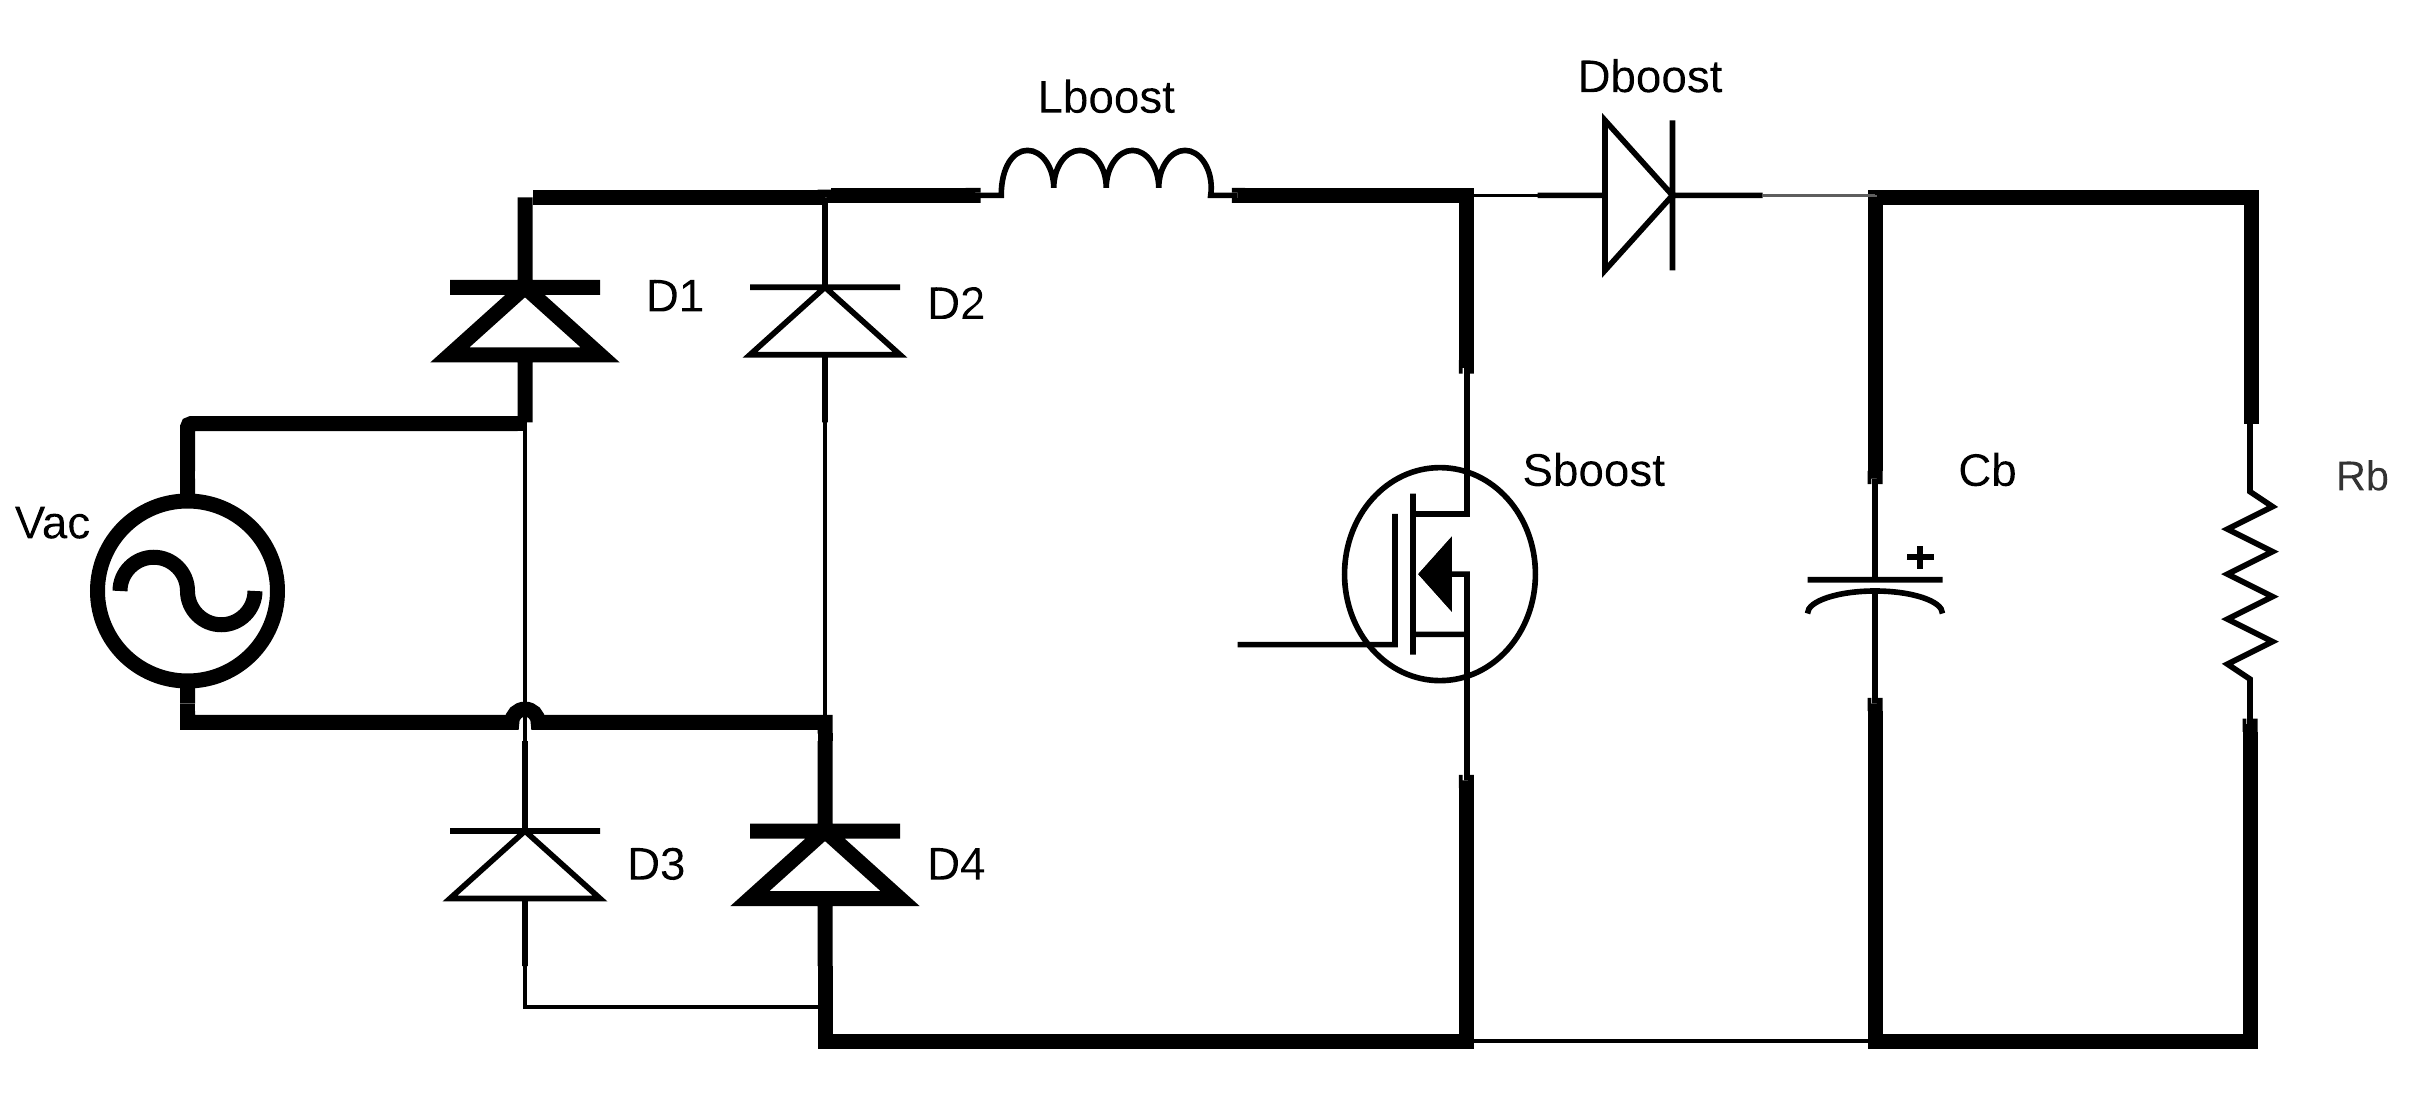
\includegraphics[width=0.5\textwidth]{figuras/energia/circuitos/1etapa_boost.png}
%\label{fig:subfig2}}
%\subfloat[][2º etapa de operação: intervalo $\Delta t_{2}$.]{
%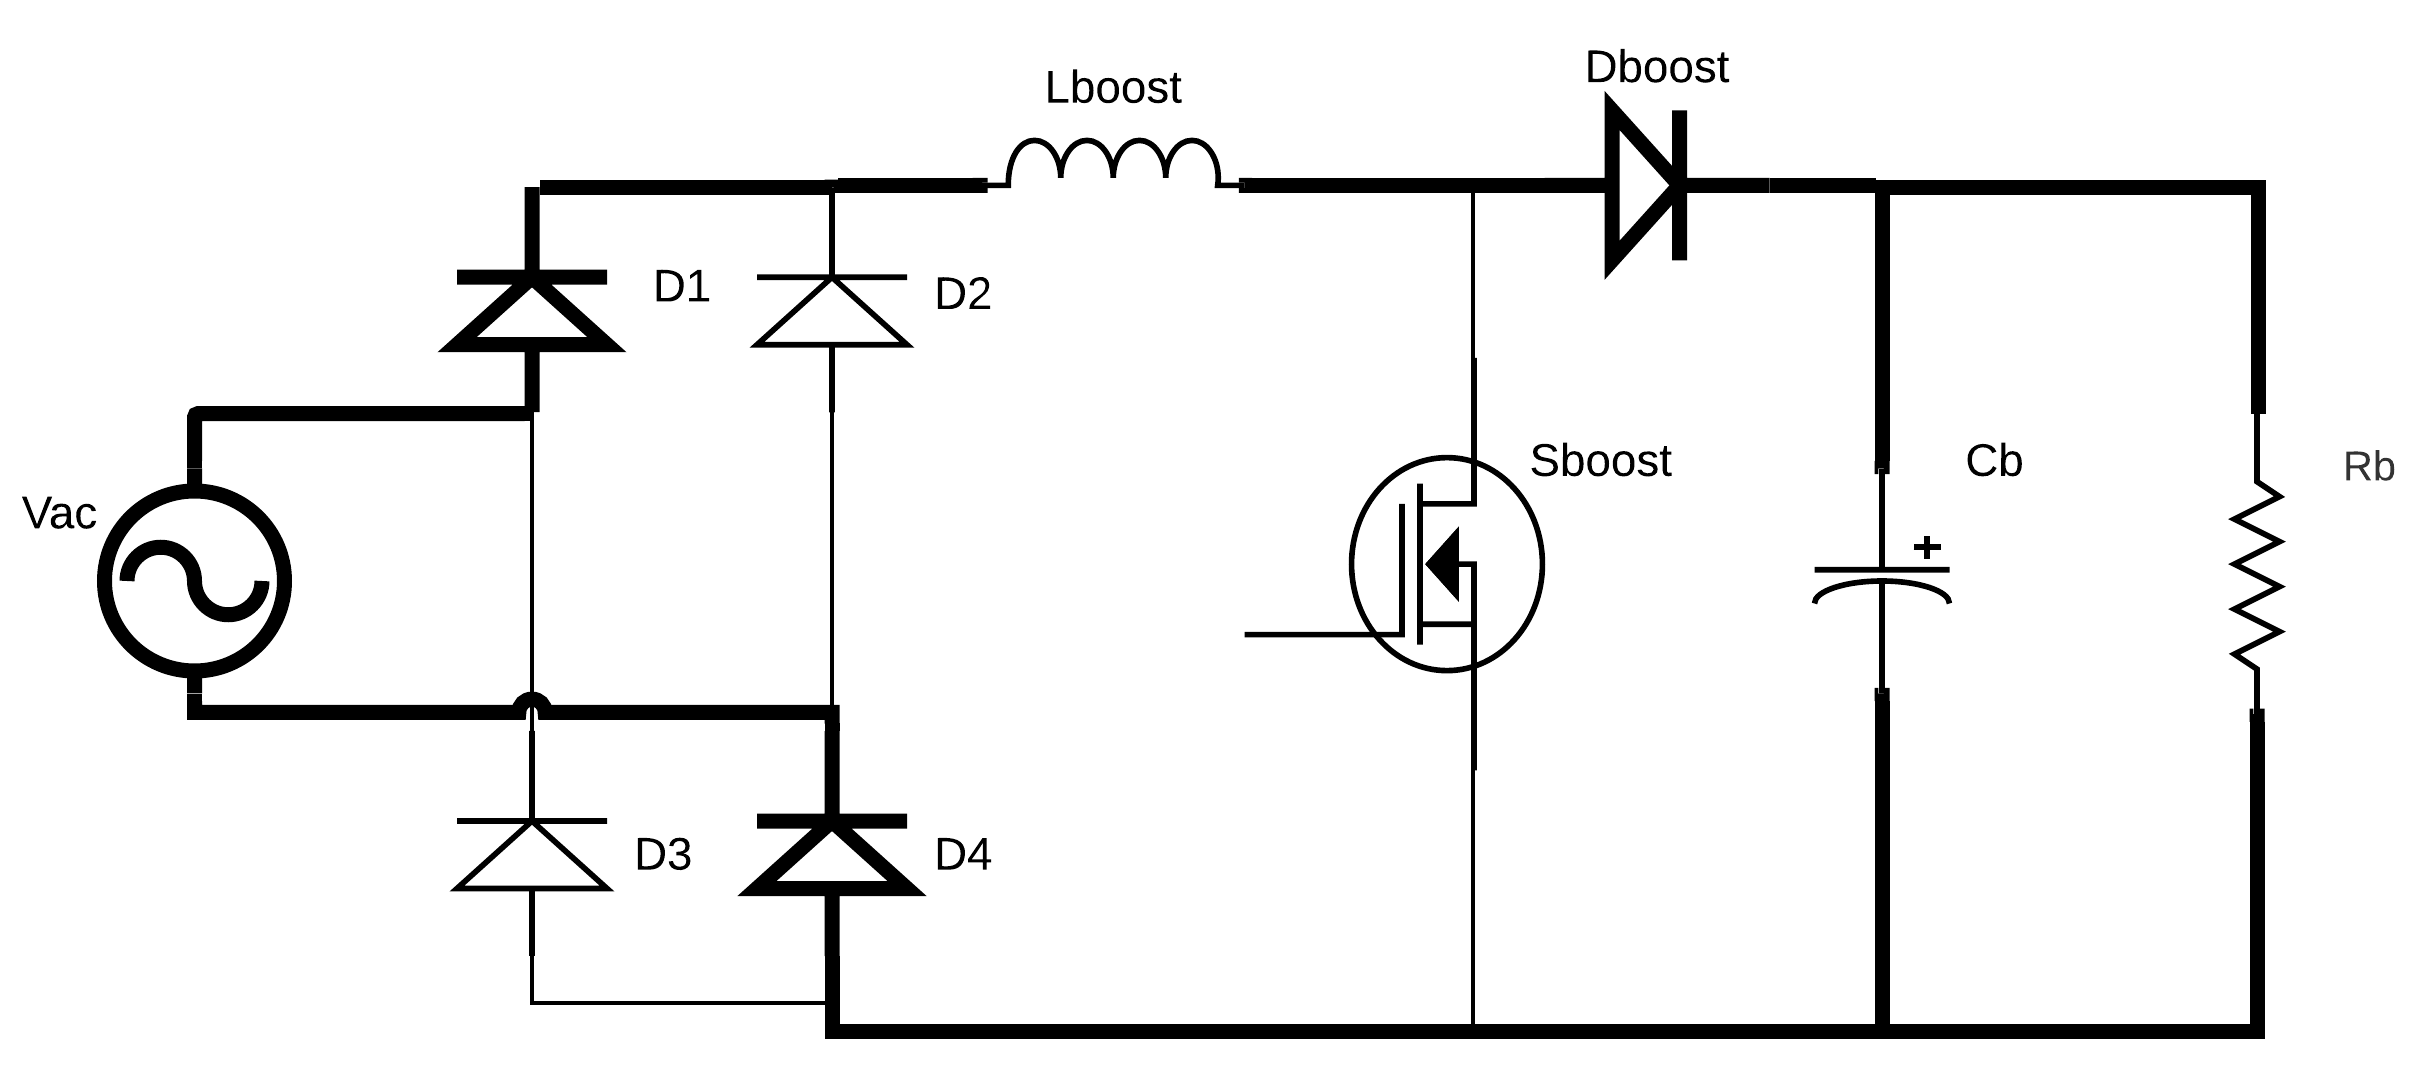
\includegraphics[width=0.5\textwidth]{figuras/energia/circuitos/2etapa_boost.png}
%\label{fig:subfig3}}
%\qquad
%\subfloat[][3º etapa de operação: intervalo $\Delta t_{3}$.]{
%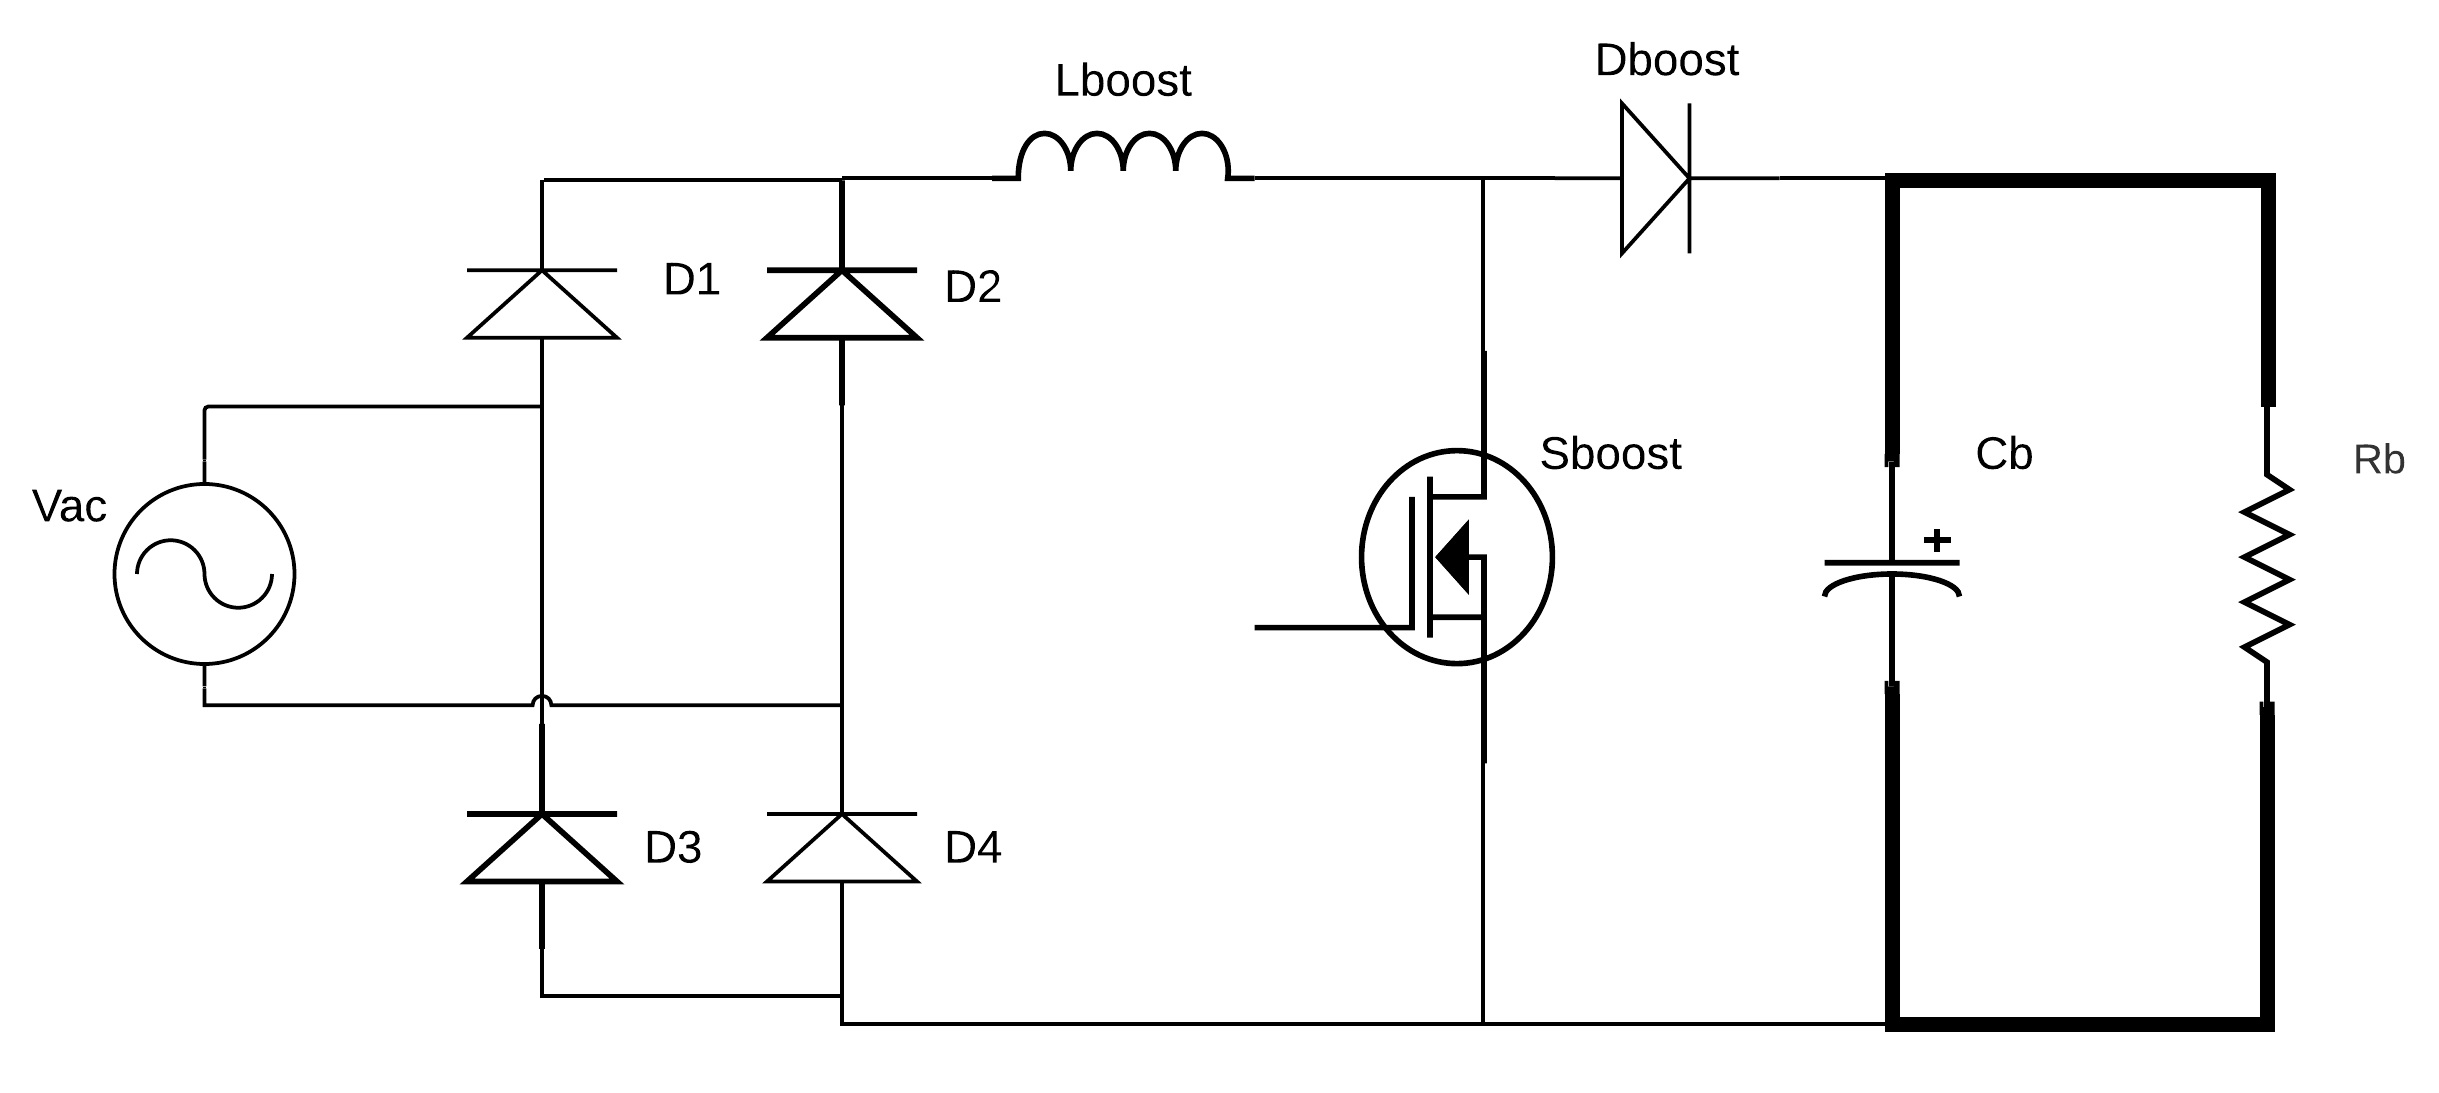
\includegraphics[width=0.5\textwidth]{figuras/energia/circuitos/3etapa_boost.png}
%\label{fig:subfig4}}
%\caption{Etapas de operação do retificador pré-regulador de fator de potência (PFP) proposto.}
%\label{fig:globfig}
%\end{figure}

%Modo de Condução Contínua (\textit{Continuous Conduction Mode} - CCM)

%O ripple (ondulação residual) de tensão resultante  
%Uma solução para a redução das perdas nessa configuração é adicionar um Transistor de Efeito de Campo de Óxido de Metal Semicondutor (MOSFET) em paralelo a cada diodo. - não será implementado 

%\begin{itemize}
   % \item \textit{Indutância ($L_{boost}$)}
    
 %   O fator de ciclo máximo é limitado de acordo com a Eq. \ref{dmax}:
    
 %   \begin{equation}
 %       D_{max} = \frac{D - 1}{D}
 %       \label{dmax}
 %   \end{equation}
    
 %   A indutância ($L_{boost}$) é calculada de acordo com a Eq. \ref{eq:indutancia}
    
 %   \begin{equation}\label{eq:indutancia}
  %      L_{boost} = \frac{V_{B}^{2} \cdot D^{2} \cdot 0,48}{2 \cdot M \cdot f_{s} \cdot P_{boost} \cdot (M-0,92)}
   %     \label{dmax}
%    \end{equation}
    
 %   O transistor ($S_{boost}$) e o diodo ($D_{boost}$) são selecionados considerando a suportabilidade da tensão reversa máxima (que é igual a tensão do barramento CC) e 
    
%\end{itemize}

\subsection{Conversor CC/CC}

Conversores CC/CC, ou \textit{choppers}, convertem a corrente contínua para uma corrente contínua em um nível de tensão diferente. A entrada para este tipo de conversor é uma tensão não regulada, portanto, seu objetivo é produzir uma tensão de saída regulada que seja adequada à carga. Na prática, é possível alcançar uma eficiência de 70\% a 95\%. O controle e regulação da tensão de saída se dá por meio da modulação por largura de pulso (\textit{Pulse-width modulation} - PWM). São utilizados dispositivos semicondutores como diodos, transistores de efeito de campo metal-óxido-semicondutor (MOSFET), transistores bipolares de porta isolada (IGBT), transistores bipolares de junção (TJB) ou tiristores. As frequências de comutação típicas estão na faixa de 1 kHz a 1 MHz, a depender da velocidade dos dispositivos semicondutores \cite{forward}.

Portanto, o conversor CC/CC produz uma tensão CC de saída cuja magnitude é controlada por meio do fator de ciclo (\textit{duty cycle}), usando circuitos auxiliares. 
%A taxa de conversão M(D) é definida como sendo a razão entre a tensão de saída CC e a tensão de entrada CC sob condições de estado estacionário \cite{forward}.

  %  \begin{equation}
   %     M(D) = \frac{V}{V_{g}}
%        \label{dmax}
 %   \end{equation}

\subsubsection*{Conversor \textit{Forward}}

Selecionar a topologia errada pode resultar em um projeto de design que não atende às suas metas de custo, metas de eficiência ou uma série de outros requisitos necessários ao projeto. Existem vários circuitos/topologias que podem aumentar ou diminuir a magnitude da tensão de saída CC e/ou inverter sua polaridade. Em muitas aplicações, é desejado incorporar um transformador no conversor de comutação, para obter uma isolação entre os circuitos de entrada e de saída, evitando, assim, choques elétricos. O tamanho e o peso do transformador variam inversamente com a frequência do sistema, portanto, as altas frequências levam a grandes reduções no tamanho do transformador \cite{forward}.

Há várias maneiras de incorporar um transformador isolador em um conversor CC/CC. O conversor isolado tipo \textit{Forward} (\textit{Buck} isolado), com um único semicondutor, é usualmente usado em fontes \textit{off-line}, na faixa de potência até 200 W e com uma alta corrente de saída. Sua configuração pode ser vista na Fig. \ref{fig:energia_forward}, onde o primário do transformador é colocado em série com um transistor ($Q_{1}$) e o enrolamento $n_{2}$ é colocado em série com o diodo $D_{1}$, a fim de desmagnetizar o núcleo do transformador ao final de cada período de comutação. O secundário do transformador é conectado a um filtro LC de saída e o diodo $D_{2}$ é inserido, de forma a prevenir uma corrente negativa no secundário do transformador  \cite{Conversores}.

\begin{figure}[H]
\centering
    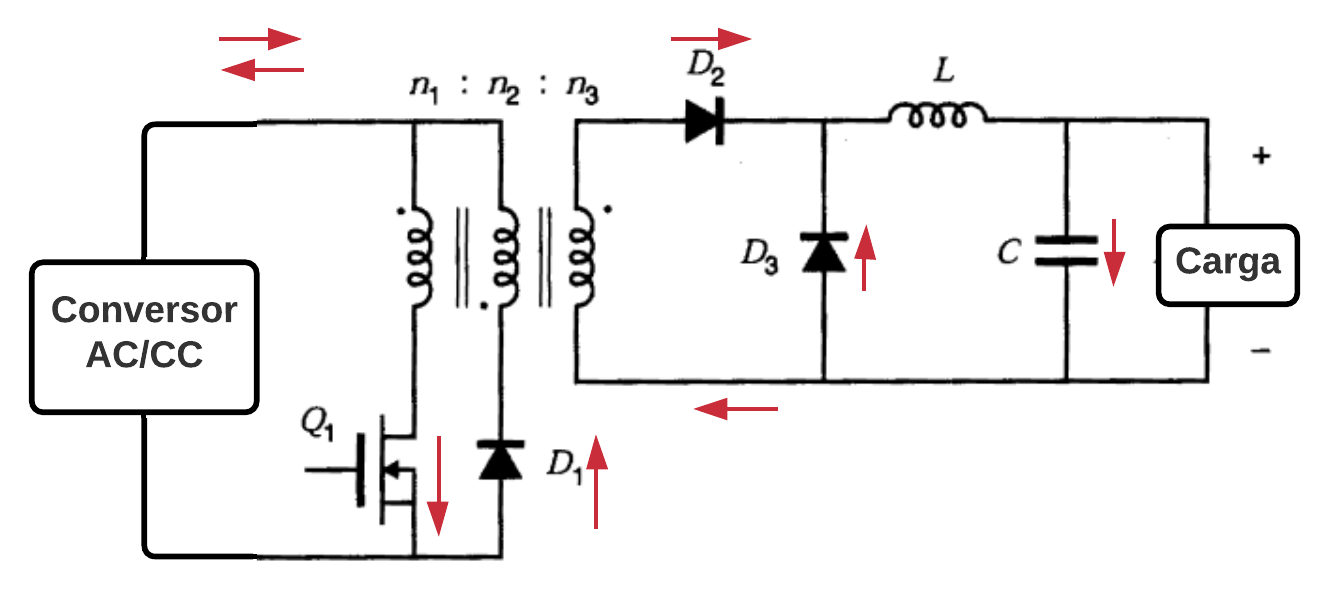
\includegraphics[width=0.8\textwidth]{figuras/energia/circuitos/Energia_forward.png}
    \caption{Configuração do conversor  \textit{Forward} com indicação do fluxo de corrente (setas vermelhas). Adaptado de: \cite{forward}}
    \label{fig:energia_forward}
\end{figure}

Suas vantagens e, portanto, a justificativa para a escolha da topologia, são \cite{Conversores}:

\begin{itemize}
    \item Isolação galvânica entre a tensão de entrada e de saída, conferindo segurança ao sistema e evitando riscos de choques elétricos durante a limpeza do equipamento. 
    
    \item Não depende de armazenamento de energia, pois a transferência de ocorre diretamente através do transformador;
    
    \item Corrente de saída de boa qualidade;
    
\end{itemize}

Dessa forma, podemos descrever a operação do retificador nas seguintes etapas:

\begin{itemize}
    \item  O transistor $Q_{1}$ conduz, junto ao diodo $D_{2}$, enquanto os diodos $D_{1}$ e $D_{3}$ estão bloqueados, situação esta em que não há corrente no enrolamento de magnetização;
    
    \item O transistor $Q_{1}$ fica bloqueado, ao passo que o diodo $D_{3}$ conduz a corrente de carga e o diodo de desmagnetização $D_{1}$ conduz a energia de volta para a fonte;
    
    \item  A corrente armazenada no indutor chega a zero, cessando a devolução de energia à fonte enquanto o diodo $D_{3}$ continua conduzindo. 
    
\end{itemize}

\begin{table}[H]
    \centering
    \footnotesize
    \caption{Parâmetros de projeto do conversor \textit{Forward}.}
    \label{Conversor_cc/cc1}
    \begin{adjustbox}{max width = \textwidth}
        \begin{tabular}{|l|c|c|}
            \hline
            \rowcolor[HTML]{A8DADC}
            \textbf{Parâmetro} & \textbf{Simbologia} & \textbf{Valor}  \\ \hline
            Tensão de Entrada & $V_{i}$ & 127-220 [V$_\text{cc}$]
            \\ \hline
           % Tensão mínima de Entrada* & $V_{CAmin}$ & 117/202 V
            %\\ \hline
            % Corrente de entrada & $I_{i}$ & X A
            %\\ \hline
            Tensão de saída & $V_{o}$ & 12 [V] 
            \\ \hline
            Corrente de saída & $I_{o}$ & 15 [A]
            \\ \hline
              Potência de saída & $P_{o}$ & 200 [W] 
             \\ \hline
              Frequência de Chaveamento & $f_{s}$ & 50 [kHz]
             \\ \hline
             %   Mínima carga & $L_{min}$ & 10 \%
             %\\ \hline
               Ondulação da Tensão de entrada (\textit{ripple}) & $\Delta V_{i(ripple)}$ & 5\%
             \\ \hline
                Ondulação da Corrente de saída (\textit{ripple}) & $\Delta I_{out(ripple)}$ & 5\%
             \\ \hline
                Rendimento & $\eta$ & 0,9
             \\ \hline
                fator de ciclo (\textit{duty cycle}) & $D$ & 0,45
             \\ \hline
                Densidade de corrente & $J$ & 450 [$\text{A}/\text{cm}^{2}$]
             \\ \hline
                 Fator de ocupação do primário & $k_{p}$ & 0,5
             \\ \hline
                 Fator de ocupação da área do enrolamento & $k_{w}$ & 0,4
             \\ \hline
                 Indução magnética & $\Delta B$ & 0,18
             \\ \hline
                  Queda de tensão no diodo & $V_{f}$ & 0,7
             \\ \hline
             \multicolumn{3}{l}{\textit{NOTA: Este design é baseado em valores típicos.}} \\ 
           % \multicolumn{3}{l}{*Valores baseados na tabela 4 (Anexo 1)
 %do módulo 8 do Prodist.} \\
        \end{tabular}
    \end{adjustbox}
\end{table}

\subsubsection*{Circuitos integradores}

Como a tensão de saída $v(t)$ do conversor é uma função do \textit{duty cycle}, um sistema de controle pode ser construído de forma que varie o \textit{duty cycle} para fazer com que a tensão de saída siga uma determinada referência. A operação deste sistema se dá da seguinte maneira: a tensão de saída é detectada usando um divisor de tensão e, então, é comparada com uma tensão CC de referência. O sinal de erro resultante é passado por uma rede de compensação em um amplificador operacional (Amp-Op), resultando em uma tensão analógica que, em seguida, é alimentada por um modulador por largura de pulso (PWM) \cite{forward}.

O modulador produz uma forma de onda de tensão comutada que controla a porta do dispositivo semicondutor. Dessa forma, o \textit{duty cycle} é proporcional à tensão analógica de controle. Essa abordagem é chamada de controle do modo de tensão. Se esse sistema de controle for bem projetado, o \textit{duty cycle} é ajustado automaticamente, de modo que a tensão de saída do conversor siga a tensão de referência e seja independente das variações da tensão de entrada ou da corrente de carga \cite{forward}.

O circuito integrador de controle PWM provê o \textit{Duty Cycle} e os elementos para implementar o controle do conversor CC/CC. O \textit{Duty Cycle} é gerado a partir de uma comparação entre o sinal triangular e sinal contínuo. Optou-se por utilizar o circuito integrado TL494 da \textit{Texas Instruments}, que é versátil e faz um ótimo trabalho ao englobar todas as etapas necessárias para o controle em um único circuito integrado.

A frequência de operação do TL494 será de 50 kHz. A frequência de trabalho do CI deve ser projetada para ser o dobro da desejada, portanto, $2 \cdot 50$ kHz = 100 kHz. Observando o gráfico da Fig. \ref{fig:chave}, utilizaremos uma capacitância de 1 nF e uma resistência de 12 k$\Omega$. Dessa forma, tem-se 50 kHz. 

\begin{figure}[H]
\centering
\subfloat[][Gráfico da frequência de oscilação \textit{versus} resistência e capacitância do CI TL494. Fonte: \textit{Datasheet} do CI TL494.]{
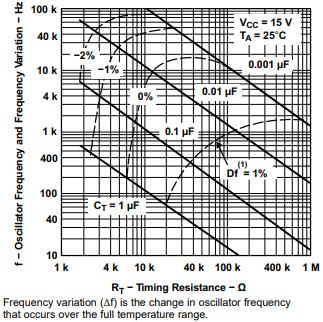
\includegraphics[width=0.3\textwidth]{figuras/energia/circuitos/chaveamento.png}
\label{fig:chave}}
\qquad
\subfloat[][Gráfico da corrente no coletor \textit{versus} corrente direta no diodo. Fonte: \textit{Datasheet} do CI TIL111.]{
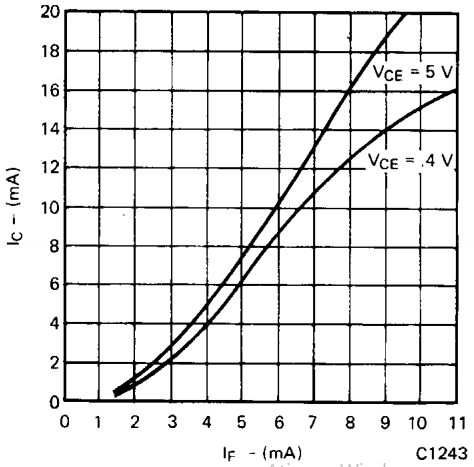
\includegraphics[width=0.3\textwidth]{figuras/energia/circuitos/isolar.png}
\label{fig:isolador}}
\caption{Gráficos dos CI's utilizados.}
%\label{fig:globfig}
\end{figure}

A isolação da realimentação do circuito é feita por meio do CI TIL111. Para saber o resistor que vai em série com o diodo emissor, foi utilizado o gráfico presente na imagem \ref{fig:isolador}. A Tab. \ref{Conversor_cc/cc2} contém os componentes selecionados para o projeto da fonte chaveada.

\begin{table}[H]
    \centering
    \footnotesize
    \caption{Componentes selecionados para o conversor \textit{Forward.}}
    \label{Conversor_cc/cc2}
    \begin{adjustbox}{max width = \textwidth}
        \begin{tabular}{|l|c|}
            \hline
            \rowcolor[HTML]{A8DADC}
          %  \multicolumn{4}{2}{Enrolamentos}  \\ \hline
            Parâmetro & Modelo/Valor Comercial
            \\ \hline
            Diodo de desmagnetização &  MUR110EG
            \\ \hline
            Diodo Série Saída &  MUR860G
            \\ \hline
            Diodo Paralelo Saída & MUR860G
             \\ \hline
              MOSFET & IRFBG20
             \\ \hline
              Capacitor & 220 uF
             \\ \hline
              Indutor & 100 uH
             \\ \hline
              Circuito de controle & CI TL494
             \\ \hline
              \textit{Feedback} Isolado & CI TIL111
             \\ \hline
              Núcleo do transformador & E-42/21/15
             \\ \hline
        \end{tabular}
    \end{adjustbox}
\end{table} 

Os componentes dos circuitos de controle e do circuito do \textit{feedback} isolado foram selecionados com base em \cite{forward2}, e estão citados na Tab. \ref{Controle}.

\begin{table}[H]
    \centering
    \footnotesize
    \caption{Componentes selecionados para o circuito de controle e do circuito do \textit{feedback} isolado do conversor \textit{Forward.}}
    \label{Controle}
    \begin{adjustbox}{max width = \textwidth}
        \begin{tabular}{|l|c|c|}
            \hline
            \rowcolor[HTML]{A8DADC}
          %  \multicolumn{4}{2}{Enrolamentos}  \\ \hline
            Parâmetro & Quant. (unid.) & Modelo/Valor Comercial
            \\ \hline
            Resistor 1/4 [W] & 1 & 680 [$\Omega$]
             \\ \hline
             Resistor 1/4 [W] & 2 & 1k [$\Omega$]
             \\ \hline
             Resistor 1/4 [W] & 1 & 1M [$\Omega$]
             \\ \hline
             Resistor 1/4 [W] & 1 & 47k [$\Omega$]
             \\ \hline
             Resistor 1/4 [W] & 2 & 5,6k [$\Omega$]
             \\ \hline
             Resistor 1/4 [W] & 1 & 10k [$\Omega$]
             \\ \hline
             Resistor 1/4 [W] & 1 & 1,5k [$\Omega$]
             \\ \hline
             Resistor 1/4 [W] & 1 & 3,3k [$\Omega$]
             \\ \hline
             Potenciômetro & 1 & 10k [$\Omega$]
             \\ \hline
             Capacitor (cerâmica) & 1 & 1 nF [$\Omega$]
             \\ \hline
             Capacitor (cerâmica) & 1 & 100 nF [$\Omega$]
             \\ \hline
        \end{tabular}
    \end{adjustbox}
\end{table} 

O apêndice \ref{Energia_memorial} contém o memorial de cálculo detalhado para o projeto e o diagrama completo da fonte, Fig. \ref{fig:diagrama_fonte2}.

\subsubsection*{Circuito abaixador de tensão}

As cargas que exigem tensão especifica no projeto são: microcontroladores, \emph{Raspberry}, visor e sensores fotoelétricos e de biometria, todos em um nível de 5 V. Somada as correntes das cargas, obteve-se 4,015 A. Portanto, necessita-se de um conversor abaixador de tensão (\textit{Step Down}). Optou-se pelo módulo regulador de tensão XL4016, com entrada de 4-40 V até 8 A e saída de 1,25 V A 36 V. 

\begin{figure}[H]
\centering
    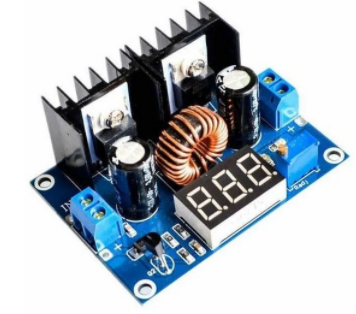
\includegraphics[width=0.4\textwidth]{figuras/energia/fotos_componentes/barramento_5V.png}
    \caption{Conversor CC/CC \textit{Step-Down} utilizado para transformar a tensão de 12 V para 5 V.}
   % \label{fig:energia_forward}
\end{figure}

\section{Sistema Autônomo de Emergência}

Nas situações em que ocorrer a interrupção na rede elétrica da concessionária, a carga do projeto será instantaneamente alimentada pelo sistema de emergência, de forma a evitar o desligamento brusco do equipamento e garantir seu funcionamento por um tempo determinado. 

A fonte primária do sistema de emergência será provida por uma bateria (acumulador de energia) e seu funcionamento se dará de maneira que, no regime de operação normal, em que as cargas são alimentadas pela fonte, a bateria estará fora de serviço. Neste mesmo regime de operação, a bateria será carregada pela fonte principal, por meio de um carregador de bateria. Haverá a comutação instantânea para a operação normal, assim que a entrada de tensão alternada (CA) seja normalizada.

A tensão nominal da bateria será igual a tensão de alimentação da carga, que foi delimitada como sendo 12 V, e os seguintes itens foram considerados para o seu dimensionamento:
%\cite{bateria}:

\begin{itemize}
    \item Autonomia do sistema (o tempo mínimo que a bateria deverá prover para que o equipamento funcione nos cenários emergenciais) igual a 1 hora;
    \item Corrente de projeto igual a 15 A, conforme estabelecido na seção \ref{section:energia_fonte};
   % \item Profundidade de descarga. A vida útil da bateria é reduzida quanto maior for a profundidade de descarga.
\end{itemize}

%Ao considerar uma autonomia da bateria (o tempo mínimo que a bateria deverá prover), de acordo com a corrente de projeto, igual a 15 A, estabelecida na seção \ref{section:energia_fonte}, de uma hora. 

Considerando carga suficiente pela disponibilidade no mercado e autonomia desejada, será utilizada uma Bateria de Lítion Íon, modelo CRG-01203M, representada na Fig. \ref{fig:energia_bateria}. A escolha dessa bateria deu-se pela alta densidade de energia e elevado potencial, baixo índice de auto-descarga e elevadas correntes de descarga \cite{STA}. Optou-se pela opção de apenas uma bateria no dispensador, para não alterar as dimensões e melhor atender o projeto. As especificações para a bateria selecionada estão contidas na Tab. \ref{Energia_bateria}.

\begin{figure}[H]
\centering
    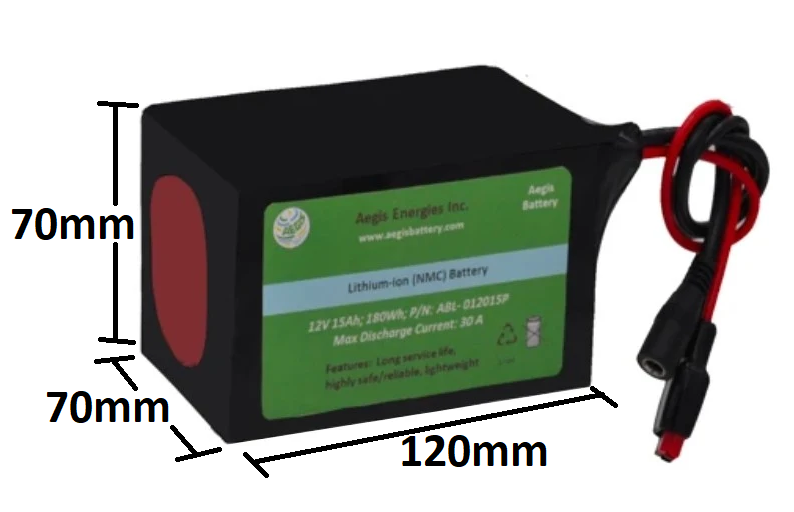
\includegraphics[width=0.4\textwidth]{figuras/energia/fotos_componentes/bateria.png}
    \caption{Bateria de Íon-Lítio, 12 V 15 Ah selecionada para o projeto.}
    \label{fig:energia_bateria}
\end{figure}

\begin{table}[H]
    \centering
    \footnotesize
    \caption{Especificações da bateria selecionada.}
    \label{Energia_bateria}
    \begin{adjustbox}{max width = \textwidth}
        \begin{tabular}{|l|c|}
            \hline
            \rowcolor[HTML]{A8DADC}
          %  \multicolumn{4}{2}{Enrolamentos}  \\ \hline
            Parâmetro & Característica
            \\ \hline
            Tipo & embalagem de PVC
            \\ \hline
            Química & íon-lítio
            \\ \hline
Dimensões  (C x L x A) & 120 x 70 x 70 [mm]
\\ \hline
 Peso & 1,05 [kg]
 \\ \hline
 Tensão de saída & 12 [Vcc]
 \\ \hline
 Capacidade/Autonomia & 15 [Ah]
 \\ \hline
 Energia armazenada & 180 [Wh]
 \\ \hline
 Vida útil & média de 1000 a 2000 ciclos
 \\ \hline
 Tempo para recarga total & até 1 hora
 \\ \hline
             Tensão de carregamento &  13,8 [V]
             \\ \hline
             corrente de carga normal & 2 [A] 
             \\ \hline
             Corrente de descarga Contínua normal & 7,5 [A]
            \\ \hline
        \end{tabular}
    \end{adjustbox}
\end{table} 

Por meio de uma verificação periódica, será possível observar o status da bateria no mostrador de cristal líquido (\textit{Liquid Crystal Display - LCD}), localizado no painel frontal da máquina, através de um indicador de carga da bateria. Este indicador apresenta:
 
 \begin{itemize}
     \item Cor verde, quando o equipamento estiver totalmente carregado;
     
     \item Cor amarela, quando o equipamento alcançar 50\% da carga total;
     
     \item Cor vermelha, quando o equipamento alcançar 25\% da carga total;
 \end{itemize}

\subsubsection*{Circuito Carregador da Bateria}
% \subparagraph*{$\bullet$ Circuito Carregador da Bateria} \hfill

O carregamento da bateria é feito automaticamente por meio de um circuito simples, que suporta uma corrente de carregamento de aproximadamente 4A. Este carregador automático realiza uma carga completa da bateria, sem danificá-la. É fundamental compreender que este circuito necessita de uma tensão superior à tensão da bateria. Para atender o projeto de carregador da bateria, foi projetado um conversor elevador de tensão CC/CC Step up 12/13,8V, representado na Fig. \ref{fig:energia_stepup}, de corrente máxima 6A,  que irá promover uma tensão superior a 12V, para que o fluxo de corrente do conversor, cuja tensão é 13,8 V, flua para a bateria 12V. O diagrama do carregamento está representado no esquemático da Fig. \ref{fig:diagrama_fonte3}.

\begin{figure}[H]
\centering
    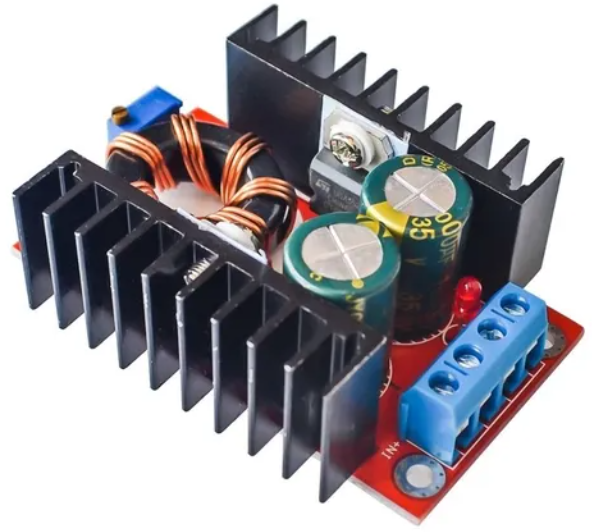
\includegraphics[width=0.4\textwidth]{figuras/energia/fotos_componentes/Energia_Stepup.png}
    \caption{Conversor Step Up 12/13,8V.}
    \label{fig:energia_stepup}
\end{figure}


\begin{table}[H]
    \centering
    \footnotesize
    \caption{Itens do circuito de carregamento da bateria.}
    \label{Itens_circuito}
    \begin{adjustbox}{max width = \textwidth}
        \begin{tabular}{|l|c|c|}
            \hline
            \rowcolor[HTML]{A8DADC}
            \textbf{Parâmetro} & \textbf{Quantidade} & \textbf{Modelo/Valor comercial}  \\ \hline
            Amplificador Operacional & 1 & UA741
            \\ \hline
            Amplificador Operacional & 1 & TIP35C
            \\ \hline
            Diodo & 1 & BZV85C55V1
            \\ \hline
             Resistor  &  2  & 470 $\Omega$
             \\ \hline
              Resistor  & 1 & 10k $\Omega$
             \\ \hline
              
                Potenciômetro & 1 & 10k $\Omega$
             \\ \hline
                Transistor & 1 & TIP35C
             \\ \hline
                Conversor Elevador & 1 & 12/13V
             \\ \hline
                      Bateria & 1 & CRG-01203M
             \\ \hline 
           % \multicolumn{3}{l}{*Valores baseados na tabela 4 (Anexo 1)
 %do módulo 8 do Prodist.} \\
        \end{tabular}
    \end{adjustbox}
\end{table}

\section{Sistema de Intertravamento entre a Fonte e a Bateria}

Para que a carga do projeto seja instantaneamente alimentada pelo sistema de emergência, de forma a evitar o desligamento brusco do equipamento e para que haja comutação instantânea para operação normal, assim que a entrada de tensão seja normalizada, necessita-se de um sistema de intertravamento entre a fonte principal e auxiliar. O acionamento do circuito de emergência se dá por meio de uma chave (relé), que tem a função de mudar a carga para o circuito alimentado pela bateria quando houver falha na fonte chaveada. O relé selecionado foi o relé reversor selado N.A/N.F – 15 A/12 V, de 5 Terminais.

Foi projetada uma placa de circuito impresso (PCI), onde a comutação para o circuito auxiliar nos casos emergenciais, carregamento da bateria e alimentação das cargas são feitas automaticamente. O diagrama do intertravamento está representado no esquemático da Fig. \ref{fig:diagrama_fonte3}.

%As proteções são essenciais para reduzir a probabilidade e as consequências das falhas. Apesar de apresentarem um custo a mais no projeto, as proteções acrescentam confiabilidade ao sistema. Para a proteção da bateria, foi utilizado um fusível de vidro 5x20 - 2,5 A 250 V, que se abre no caso de uma corrente excessiva. 

\subsection{Dimensionamento da PCI}

A placa de circuito impresso (PCI) do diagrama do carregamento e do intertravamento está representada na Fig. \ref{fig:PCB_energia}. Para a confecção da PCI, foi seguido o plano de construção descrito na seção \ref{sec:plano_de_construção} da solução eletrônica. Considerando uma placa com 3 onças de espessura de cobre e uma corrente máxima de 15 A, temos que a área da seção transversal é igual a 682,0 $\text{mils}^2$ e a largura da trilha é igual a 165,35 mils. Para o projeto da PCI, considerou-se uma folga na largura, portanto, selecionou-se 200 mils, o que corresponde a 5 mm. Foi utilizado uma zona preenchida de \textit{Ground} (GND) na camada de cobre e conectores borne para as seguintes conexões na parte superior:

\begin{itemize}
    \item Conversor \textit{Step-Up} 12 V/13,8 V;
    
    \item Bateria íon-lítio;
    
    \item Fonte de alimentação 110-220 V/12 V;
    
    \item Três blocos terminais de fios que se conectam com as cargas. 
\end{itemize}

Para as conexões, são utilizados cabos flexíveis de cobre com bitola de 2,5 $[\text{mm}^2]$. 

\begin{figure}[H]
    \centering
    \subfloat[][Trilhas da PCI frente]{
    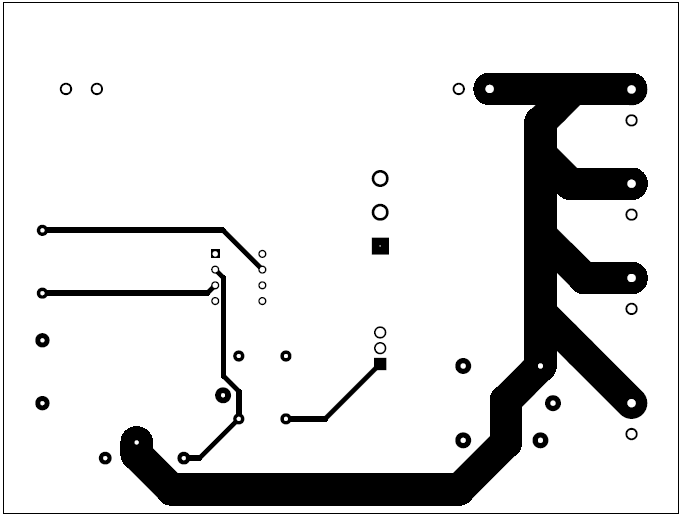
\includegraphics[width=4.4cm]{figuras/energia/circuitos/PCB_1.PNG}
   % \label{fig:trilhas_2_m11}
    }
    \subfloat[][Trilhas da PCI verso]{
    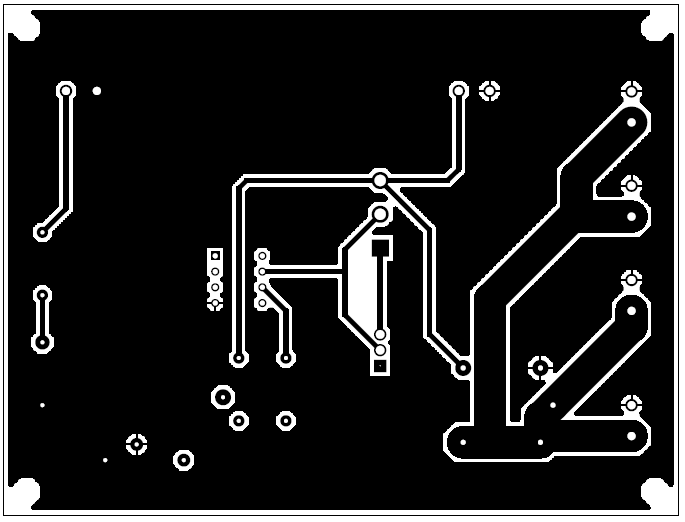
\includegraphics[width=4.4cm]{figuras/energia/circuitos/PCB_2.PNG}
    %\label{fig:trilhas_2_m112}
}
    
    \subfloat[][Vista superior da PCI]{
    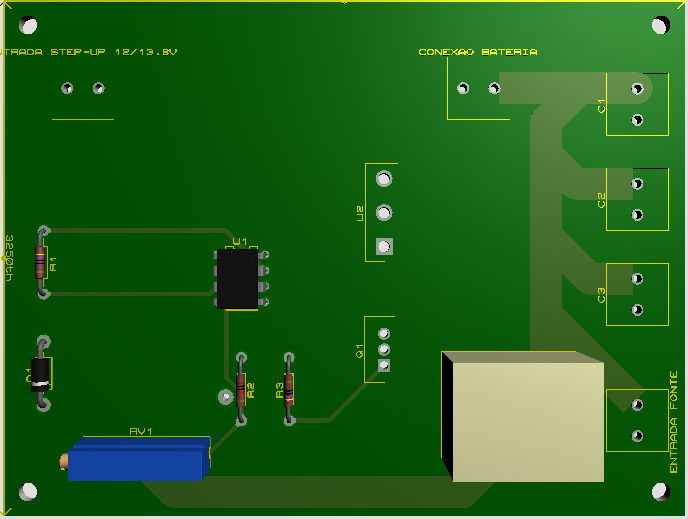
\includegraphics[width=4.4cm]{figuras/energia/circuitos/PCB bateria front.PNG}
    \label{fig:energia_3D_2_m12}}
    \subfloat[][Vista inferior da PCI ]{
    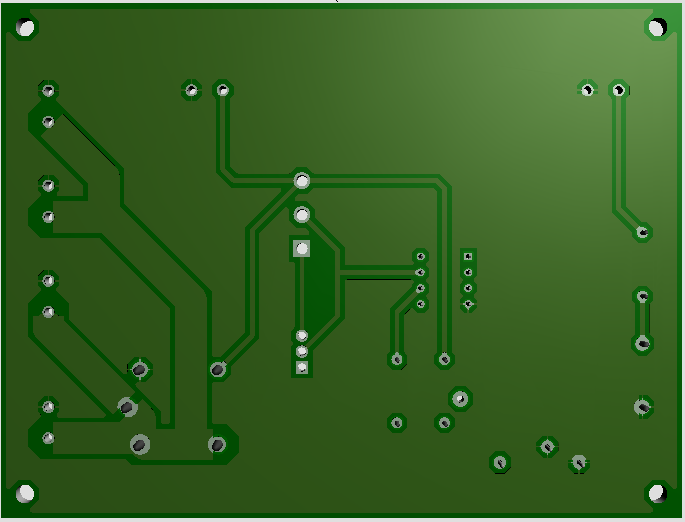
\includegraphics[width=4.4cm]{figuras/energia/circuitos/PCB bateria back.PNG}
    \label{fig:energia_3D_3_m13}}
    \caption{PCI carregamento da bateria e intertravamento entre bateria e fonte.}\label{fig:PCB_energia}
\end{figure}


\section{Dimensionamento dos Condutores}
\label{section:energia_cabos}
%tabela 47 e 38 NBR 5410

O dimensionamento dos condutores foi realizado com base na norma NBR 5410/2004. O objetivo principal desta norma é estabelecer condições que instalações elétricas de baixa tensão devem satisfazer, a fim de garantir a segurança de pessoas e animais, assim como o funcionamento adequado da instalação e conservação dos bens presentes no local. 

\begin{enumerate}
    \item Método 1: Seção referente a uma análise das condições apresentadas pela norma, de acordo com o tipo de linha e utilização do circuito. 
    
    \item Método 2: Seção referente a escolha da corrente nominal do projeto, em que, para cada circuito, terá uma seção específica de condutor. 
\end{enumerate}

De acordo com a norma, os métodos de referências são os métodos de instalação para os quais a capacidade de condução de corrente foi determinada, por ensaio ou por cálculo. A referência utilizada no projeto foi o F: cabos unipolares justapostos ao ar livre. Para fins de dimensionamento dos condutores, são considerados os seguintes circuitos:

\begin{itemize}
    \item Circuito A: entrada da rede;
    
    \item Circuito B: saída da fonte/bateria;
    
    \item Circuito C: motores de passo;
    
    \item Circuito D: atuador elétrico;
    
    \item Circuito E: atuador \textit{push-pull};
    
    \item Circuito F: motor DC (esteira);
    
    \item Circuito G: componentes eletrônicos.
\end{itemize}

De acordo com a Tab. 47 da NBR 5410/2004, para o método 1, os circuitos de tomadas de corrente são considerados circuitos de força, portanto, os circuitos A, B, C, D, E, F e G são considerados de força. O método 2 depende da corrente de projeto do circuito, de forma que a capacidade de condução de corrente dos condutores deve ser igual ou superior à corrente de projeto. A corrente de projeto ($I_{projeto}$) é calculada de acordo com a Eq. \ref{energia_corrente1}, onde é considerada um rendimento ($\eta$) de 100\%, um fator de potência (FP) unitário e queda de tensão inferior a 4\%. A seção final dos condutores é dada pela maior seção entre os dois parâmetros encontrados, e o resultado está contido na Tab. \ref{energia_seção}.
    
    \begin{equation}
        I_\text{projeto} = \frac{P_\text{circuito} \cdot 1,2}{V \cdot FP \cdot \eta} \quad [\text{A}]
        \label{energia_corrente1}
    \end{equation}
    %\left(  \right)}

\begin{table}[H]
    \centering
    \footnotesize
    \caption{Determinação da seção dos condutores.}
    \label{energia_seção}
    \begin{adjustbox}{max width = \textwidth}
        \begin{tabular}{|c|c|c|c|c|c|}
            \hline
            \rowcolor[HTML]{A8DADC}
          %  \multicolumn{4}{2}{Enrolamentos}  \\ \hline
            Circuito & Potência (W) & Corrente de projeto (A) & Método 1 ($mm^{2}$)& Método 2 ($mm^{2}$)& Seção escolhida ($mm^{2}$)
            \\ \hline
            A  & 222 & 1,21 & 2,5 & 0,5 & 2,5
            \\ \hline
             B & 180 & 18 & 2,5 & 1,5 & 2,5
            \\ \hline
             C & 4,8 & 0,4 & 2,5 & 0,5 & 2,5
            \\ \hline
             D & 24 & 2 & 2,5 & 0,5 & 2,5
            \\ \hline
             E & 5,6 & 1,12 & 2,5 & 0,5 & 2,5
            \\ \hline
             F & 19,2 & 1,6 & 2,5 & 0,5 & 2,5
            \\ \hline
             G & 74,34 & 7,43 & 2,5 & 0,5 & 2,5
            \\ \hline
        \end{tabular}
    \end{adjustbox}
\end{table}

\subsection{Plugue e Conectores}

A norma IEC 61140 dispõe os tipos de conexão do equipamento eletrônico com a terra. A proteção contra choques elétricos nesses equipamentos se dá por meio da medida de segurança conhecida como classe de isolamento. O equipamento Pill Watcher está classificado como Classe I, onde sua carcaça é metálica e está conectada à terra através de um condutor de proteção (PE). Com isso, de acordo com o Padrão Brasileiro de Plugues e Tomadas, o modelo de plugue do equipamento é de três pinos e a tomada a que ele for conectado deve ser de três orifícios de 4,8 mm, pois a corrente do projeto é de 20A.

Com base na classificação estabelecida na norma IEC 61140 para o equipamento Pill Watcher, o plugue utilizado no projeto é o modelo 108-1MR, da marca Cabosata, com corrente máxima de 20 A e tensão de até 300/500 V. Este apresenta três fios internos de 2,50 mm e um plugue macho de pinos redondos de 4,8 mm.  

Os conectores elétricos são dispositivos eletromecânicos que fazem ligações elétricas entre condutores, configurados para eliminar ou reduzir fugas de corrente provocadas por emendas ou outros tipos de conexões.  Sua função é conectar duas ou mais partes de um mesmo fio. Evitam perda de energia elétrica e consumo desnecessário quando dimensionados e instalados corretamente para os fios. 

Para o sistema de alimentação, ocorreram as seguintes conexões:


\begin{itemize}

      \item Para a conexão com os cinco motores de passo, são utilizados 5 cabos com conexão Molex KK de 4 pinos macho/fêmea conectados no conector do drive A4988.
    \item Para a conexão com motor DC, é utilizado um cabo com conexão Molex KK de 2 pinos macho/fêmea conectado no conector do drive L298N.
    \item Para a conexão com o atuador elétrico, é utilizado um cabo com conexão Molex KK de 2 pinos macho/fêmea conectado no conector do drive IRF520N.
     \item Para a conexão com as 25 solenoides, são utilizados 25 cabos com conexão Molex KK de 2 pinos macho/fêmea conectado no conector do drive IRF520N.
    \item Para a conexão com as 7 fechaduras solenoides, são utilizados 7 cabos com conexão Molex KK de 2 pinos macho/fêmea conectado no conector do drive IRF520N.
    \item Para a conexão da PCI de intertravamento e carregamento da bateria, foram utilizados 6 conectores Borne KRE com 2 pinos conectados ao conector da bateria, conversor step, fonte e borne.
     
\end{itemize}

  

 
% \begin{table}[H]
 %   \centering
  %  \footnotesize
   % \caption{xxxxxx }.
    %\label{Conectores_Pugles}
    %\begin{adjustbox}{max width = \textwidth}
     %   \begin{tabular}{|l|c|}
      %      \hline
       %     \rowcolor[HTML]{A8DADC}
        %  %  \multicolumn{4}{2}{Enrolamentos}  \\ \hline
    %        Parâmetro & Quantidade
     %       \\ \hline
      %      Conector Mulex KK &  x
       %     \\ \hline
        %    
        %\end{tabular}
    %\end{adjustbox}
%\end{table}  

\section{Elementos de Organização}

O processo de organização dos cabos envolveu a definição de prioridades para que o ambiente do equipamento tenha um visual organizado. Portanto, seguiu-se os seguintes passos:

\begin{enumerate}
    \item Determinação das posições fixas dos elementos na estrutura do equipamento;
    
    \item Verificação das necessidades dos cabos para cada circuito;
    
    \item Etiquetação dos cabos para identificação dos circuitos;
    
    \item Diminuição dos cabos, sempre que possível;
    
    \item Definição dos caminhos dos cabos na estrutura para facilitar a montagem e desmontagem do equipamento;
\end{enumerate}

Por meio da Fig. \ref{fig:energia_cabos}, onde os círculos rosas representam as posições das solenoides e motores de passo, foi possível calcular as distâncias de cada circuito (A1, A2...), desde à posição inicial da fonte e da bateria. Com isso, obtemos os comprimentos necessários para os cabos de alimentação dos circuitos, que se encontram resumidos na Tab. \ref{tab:energia_cabos}.

\begin{figure}[H]
    \centering
    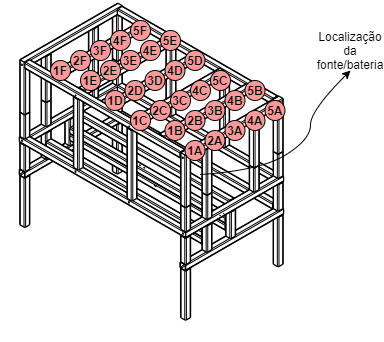
\includegraphics[width=0.5\textwidth]{figuras/energia/circuitos/cabos.png}
   \caption{Identificação dos circuitos para dimensionamento das distâncias dos condutores.}
   \label{fig:energia_cabos}
   \end{figure}
   
\begin{table}[H]
    \centering
    \caption{Distância, em metros, dos condutores tendo como referência a Fig. \ref{fig:energia_cabos}.}
    \label{tab:energia_cabos}
    \begin{adjustbox}{max width = \textwidth}
    % \begin{adjustwidth}{-2,5cm}{}
        \begin{tabular}{|>{\columncolor[HTML]{A8DADC}}c|l|c|c|c|c|c|}
            \hline
            \rowcolor[HTML]{A8DADC}
         &\multicolumn{1}{c|}{\textbf{A}} & \multicolumn{1}{c|}{\textbf{B}} & \multicolumn{1}{c|}{\textbf{C}} & \multicolumn{1}{c|}{\textbf{D}} & \multicolumn{1}{c|}{\textbf{E}} & \multicolumn{1}{c|}{\textbf{F}}
        \\ \hline 
          \textbf{1}  & 1.8 & 1.6 & 1.4 & 1.6 & 1.8 & 2.0
          \\ \hline 
          \textbf{2}  & 1.6 & 1.4 & 1.2 & 1.4 & 1.6 & 1.8
          \\ \hline
          \textbf{3}  & 1.4 & 1.2 & 1.0 & 1.2 & 1.4 & 1.6
          \\ \hline
          \textbf{4}  & 1.2 & 1.0 & 0.8 & 1.0 & 1.2 & 1.4
          \\ \hline
          \textbf{5}  & 1.0 & 0.8 & 0.6 & 0.8 & 1.2 & 1.2
          \\ \hline

            \end{tabular}
    % \end{adjustwidth}
    \end{adjustbox}
\end{table}

 
Para o circuito do atuador elétrico, o caminho determinado para a passagem dos condutores, de forma segura, possui uma distância igual a 0,6 metros. Para o circuito do motor DC, o caminho determinado para passagem dos condutores, de forma segura e com disponibilidade de espaço, sua distância é igual a 0,9 metros. 
\subsection{Barramento de Distribuição}

A alimentação do conjunto de cabos a serem distribuídos para cada dispositivo na estrutura do \textit{Pill Watcher} é feita por meio de blocos terminais de fios, que são um conjunto de pontos de conexão aparafusados semelhantes que garantem uma maneira segura e conveniente para manter organizados a fiação dentro da estrutura. Dessa forma, uma tira de terminais combina muitos blocos semelhantes em um único dispositivo. 

As principais funções de um bloco de terminais são conectar e isolar. O corpo do bloco principal é feito de um material resistente, neste caso plástico, que isola eletricamente os blocos adjacentes, e suas partes condutoras são feitas de cobre resistente à corrosão. Em uma faixa, os blocos são isolados uns dos outros, como pode ser visto na Fig. \ref{fig:energia_bloco} para o bloco terminal selecionado para a solução, este possui um ângulo entre a entrada e saída de fios igual a 90°.

\begin{figure}[H]
\centering
\subfloat[][]{
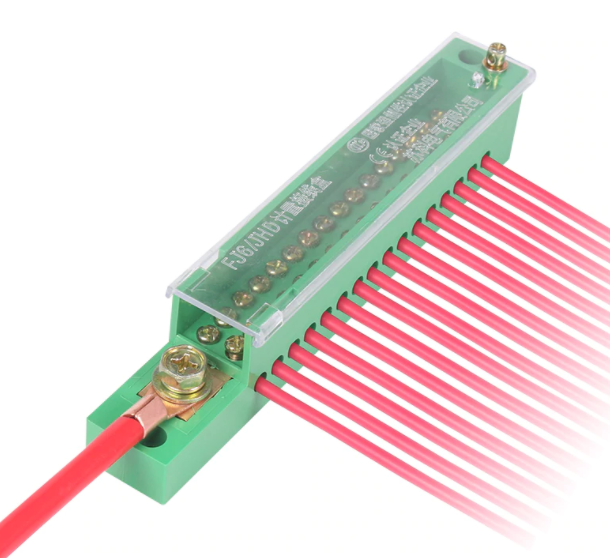
\includegraphics[width=0.4\textwidth]{figuras/energia/fotos_componentes/borne_1.PNG}
%\label{fig:ch}
}
\qquad
\subfloat[][]{
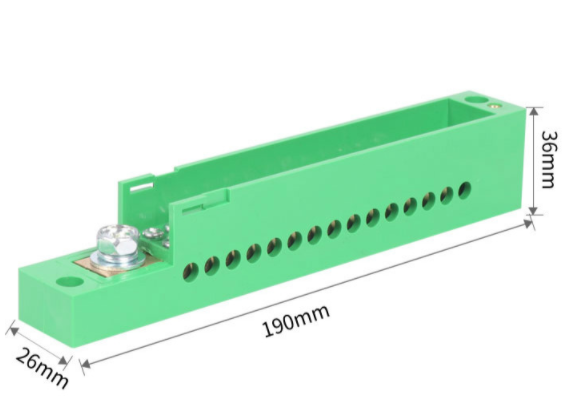
\includegraphics[width=0.4\textwidth]{figuras/energia/fotos_componentes/borne_2.PNG}
%\label{fig:isolador}
}
\caption{Bloco terminal de fio.}
\label{fig:energia_bloco}
\end{figure}

Para a aplicação, foi considerado o número de fios necessários para o projeto para, então, obter o número de contatos necessários. Dessa forma, considerando os circuitos de A à G, definidos na seção \ref{section:energia_cabos}, temos que o número de fios requeridos para a saída da fonte é igual a 42. Combinando 6 blocos, do bloco representado na Fig. \ref{fig:energia_bloco}, tem-se 48 contatos disponíveis. Dos 6 blocos, 3 são para o potencial positivo da corrente contínua de saída e 3 para o potencial negativo. O esquema de etiquetagem definido no processo de organização dos cabos, Fig. \ref{fig:diagrama_etiqueta}, se deu após a definição das posições fixas dos elementos na estrutura, e permite identificar como os fios são organizados. Os 6 blocos são fixados na chapa da estrutura em que estão dispostos a fonte e a bateria. 

\begin{figure}[!htb]
    \centering
    %\vspace{2cm}
     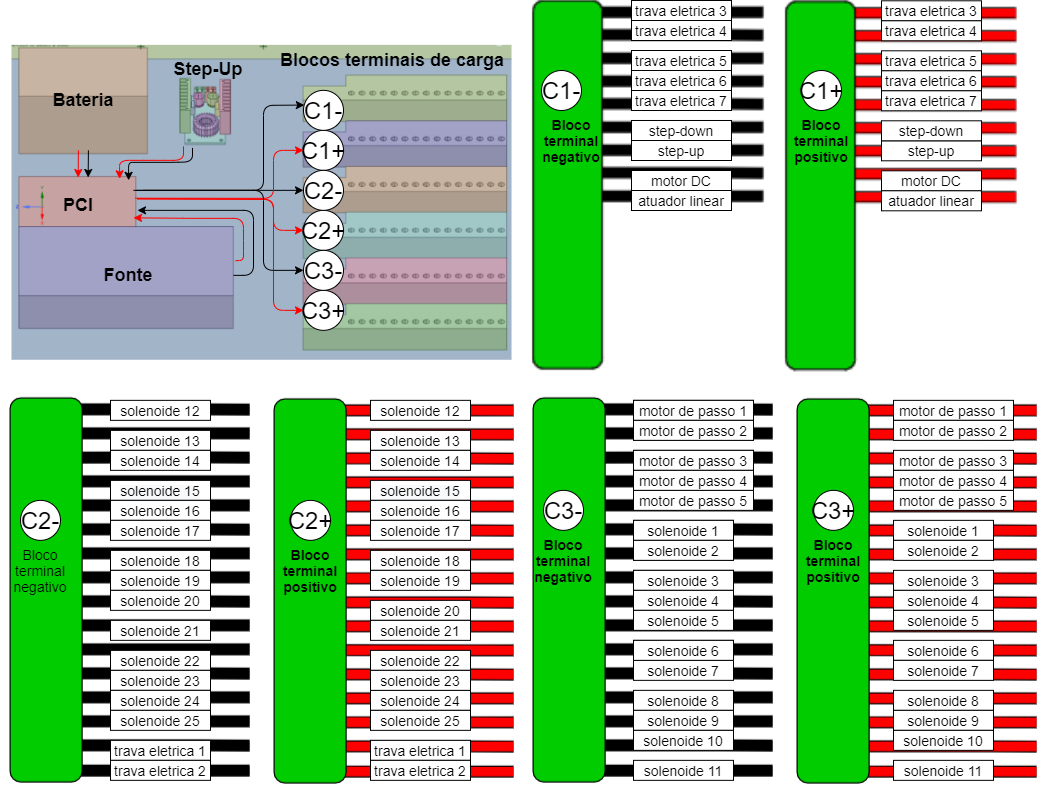
\includegraphics[width=1\textwidth, height=2\textheight,keepaspectratio]{figuras/energia/diagramas/etiquetagem.png}
    \caption{Identificação dos Circuitos nos Blocos Terminais de Fio.}
    \label{fig:diagrama_etiqueta}
\end{figure}

\subsection{Proteção e Acabamento}
\label{energia_subseção_cabos}

Optou-se por utilizar canaletas de PVC (Cloreto de Polivinil) com recorte aberto para a organização dos fios e cabos da alimentação e da comunicação entre os dispositivos. Esta configuração evita que os fios fiquem amontoados e protege mecanicamente os cabos contra danos externos. A canaleta recorte é composta por duas partes: uma que tampa e outra que vai fixada na superfície desejável. Este tipo de canaleta possui uma abertura lateral, onde o rasgo vai até o encaixe da canaleta, possibilitando a derivação de fios em qualquer ponto.

Após a escolha das superfícies onde serão fixadas as canaletas, é necessário escolher uma largura da canaleta que caiba na superfície a ser fixada e que tenha espaço suficiente para abrigar os cabos. A superfície na estrutura em que será fixada as canaletas serão os tubos estruturais, que possuem uma largura de 50,8 mm. Para o dimensionamento e seleção da canaleta, levou-se em consideração a relação dos cabos do caminho na estrutura que levará a maior quantidade de cabos, a seção total dos condutores e a capacidade de suportar as solicitações mecânicas, químicas, elétricas e térmicas a que for submetida, nas condições da instalação. 

De acordo com a NBR 5410/2004, as canaletas instaladas sobre superfícies devem ser escolhidas e dispostas de modo a não danificar os cabos nem comprometer seu desempenho. Tendo em vista que todos os condutores dos circuitos possuem uma seção nominal de 2,5 $\text{mm}^2$, considerou-se que a seção útil de um condutor e seu diâmetro máximo são, respectivamente, 13,9 $\text{mm}^2$ e 4,2 $\text{mm}^2$. A descrição dos cabos para o caminho que levará a maior quantidade cabos, é, portanto:

\begin{enumerate}
    \item 10 cabos para a alimentação do circuito dos motores de passo;
    \item 50 cabos para a alimentação do circuito das solenoides;
    \item 14 cabos para a alimentação do circuito da fechadura elétrica.
\end{enumerate}

Totalizando 74 cabos. Dessa forma, o cálculo das secções acumuladas dos cabos é 74 x 13,9 $\text{mm}^2$ = 1028,6 $\text{mm}^2$. Com isso, foi escolhida a canaleta, em função do volume ocupado pelos cabos, que possui 30 mm de largura, 50 mm de altura e que trabalha em uma temperatura entre -40 a 85°C. Esta encontra-se representada na Fig. \ref{fig:energia_canaleta}. A área de sua seção transversal é igual a 1500 $\text{mm}^2$, portanto, a disposição dos cabos no interior atende à área disponível da canaleta escolhida, considerando uma certa folga. 

\begin{figure}[H]
\centering
    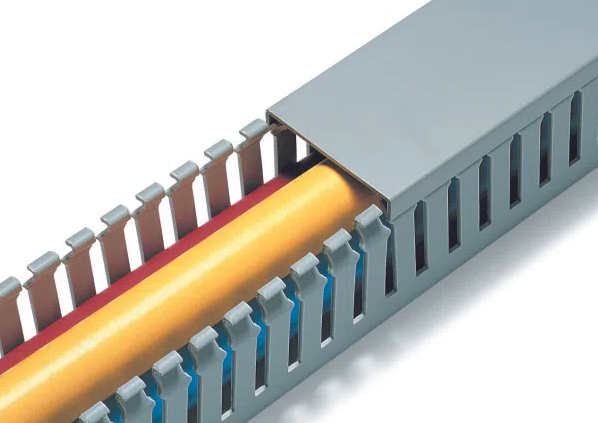
\includegraphics[width=0.4\textwidth]{figuras/energia/fotos_componentes/canaleta.png}
    \caption{Canaleta recorte aberto.}
    \label{fig:energia_canaleta}
\end{figure}

Ao definir o caminho a ser percorrido pelas canaletas, desde a saída dos blocos terminais de fio até às cargas, calculou-se uma distância total de 8,29 metros, arredondada para 9 metros. As canaletas possuem furos em sua base, para serem fixadas na estrutura a cada 50 mm. Com a distância de 9 metros determinada, necessita-se que o caminho proposto tenha 180 furos, com 50 mm de distância entre eles. As canaletas são fixadas por elementos chamados fixa-dutos, que oferecem segurança e praticidade na instalação no projeto. Necessita-se, portanto, de 180 fixa-dutos. 


% 1 motor de passo 0,5mm²

%O primeiro parâmetro é uma análise das condições apresentadas pela norma, de acordo com o tipo de linha e utilização do circuito. Como o circuito geral do dispensador contem motores e componentes eletrônicos, a utilização do circuito é classificada como de força. Como o sistema de alimentação apresenta uma fonte que mudará a tensão de entrada,o dimensionamento dos condutores foi realizado para os cabos de entrada rede elétrica (220V), saída da fonte (12V), para os motores (circuito A) e equipamentos eletrônicos(circuito B). 

%A seção final dos condutores é dada pela maior seção entre os dois parâmetros encontrados. Desse modo, de acordo com a Tab. 47 da NBR 5410/2004 tem-se que a seção mínima dos condutores de entrada, para os circuitos A é Ymm(Cu) e para o circuito B, Xmm. 

\section{Sistema de proteção}

O fusível é um dispositivo de proteção contra sobrecorrente, que opera quando houver uma sobrecarga ou curto-circuito no sistema, evitando, assim, danos no isolamento dos condutores e/ou nos componentes do \textit{Pill Watcher}. Este deve ser dimensionado para uma corrente, no mínimo, 20\% maior que a corrente de operação do circuito que irá proteger.

    \begin{equation}
        I_\text{fusível} = 1,2 \cdot \frac{P_\text{operação}}{V_{N} \cdot FP \cdot \eta} = \frac{222 \cdot 1,2}{110 \cdot 1 \cdot 1} = 2,42 \quad [\text{A}]
        \label{energia_corrente2}
    \end{equation}
    %\left(  \right)}
    
Para o cálculo da Eq. \ref{energia_corrente2}, foi considerada a tensão de entrada igual a 110 V, pois é a situação mais crítica. A categoria de utilização do fusível será a G, para a proteção de linha que atuará na presença tanto de curto-circuito como de sobrecarga. Foi selecionado um fusível de vidro 5x20 - 2,5 A 250 V. 

\section{Plano de Testes}\label{sec:plano_teste_energia}

O plano de testes do subsistema de alimentação consistirá na medição dos seus parâmetros de operação, de modo a verificar se o sistema está atendendo os parâmetros propostos. 

\subsection{Teste da Fonte}
O primeiro teste a se realizar na fonte é o teste de circuito aberto. Primeiramente, conecta-se a fonte a uma tomada de 220 volts e verifica-se, com um voltímetro, se a tensão de saída da fonte é de 12 Vdc estáveis. O mesmo procedimento deve ser realizado com uma tomada de 110 volts, na medida em que a tensão de saída deverá também ser de 12 Vdc.

O segundo teste consiste em verificar a tensão e a corrente de saída em plena carga, ou seja, de acordo com o que foi estabelecido no cenário 4 indicada no item 7.2 deste projeto. Para a execução deste teste, faz-se uso de um circuito de carga equivalente à indicada no cenário 4, ou do mesmo testador multifuncional utilizado no teste da bateria adotada para o Pill Watcher. A tensão e a corrente de saída devem se manter constantes e sem oscilações superiores a 5\% em relação a 12 Vdc e 9A, respectivamente.

\subsection{Teste da Bateria}
O teste da bateria escolhida para o equipamento Pill Watcher será realizado com auxílio de um testador multifuncional de baterias, que verificará a capacidade de armazenamento da bateria e o tempo de descarga, quando submetida a uma carga constante.

O teste consiste em configurar a corrente da carga para 15A no testador, e aguardar que o testador descarregue a bateria por completo. O tempo medido pelo testador não deve ser inferior a 1 hora.

\subsection{Teste do Sistema de Carregamento}
O teste do sistema de carregamento consiste em verificar quanto tempo este sistema necessita para carregar completamente a bateria e se o fluxo de corrente é interrompido, quando a bateria está plenamente carregada. 

Para a execução deste teste, conecta-se uma bateria completamente descarregada e mede-se o fluxo de corrente que flui do Sistema de Carregamento para a bateria. Os valores típicos de corrente especificados são da ordem de 2A, tendendo a zero quando completo o carregamento da bateria. O tempo esperado para o carregamento da bateria nessas condições é de 1 hora e deve ser medido durante a fase de teste do sistema de carregamento.

\subsection{Teste do Intertravamento}
O teste do intertravamento consiste em averiguar a tensão de saída desse sistema, quando há ocorrência de queda na tensão na fonte de tensão de entrada.

Para execução desse teste, recomenda-se o uso de uma fonte de tensão alternada regulável, conectada à entrada da fonte do \textit{Pill Watcher}, e de um osciloscópio, conectado à saída do sistema de intertravamento. 

A fonte do \textit{Pill Watcher} e a bateria carregada devem estar conectados ao sistema de intertravamento.

O plano de teste deste sistema consiste nas seguintes etapas:

\begin{itemize}

              \item Regular a fonte de tensão alternada para 220 V na entrada da fonte do \textit{Pill Watcher} e verificar, no osciloscópio, se a tensão de saída do sistema de intertravamento é de 12 Vdc;
              \item Reduzir bruscamente a tensão alternada para 110 V na entrada da fonte do \textit{Pill Watcher} e verificar, no osciloscópio, se a tensão de saída do sistema de intertravamento é de 12 Vdc. É importante verificar se não há oscilações superiores a 5\% na tensão de saída observada no osciloscópio.
             \item Reduzir bruscamente a tensão alternada para 50 V na entrada da fonte do \textit{Pill Watcher} e verificar, no osciloscópio, se a tensão de saída do sistema de intertravamento é de 12 Vdc. Neste momento, o suprimento de energia do \textit{Pill Watcher} se dará exclusivamente pela bateria. É importante verificar se não há oscilações superiores a 5\% na tensão de saída observada no osciloscópio.
             \item Aumentar bruscamente a tensão alternada para 220 V na entrada da fonte do \textit{Pill Watcher} e verificar, no osciloscópio, se a tensão de saída do sistema de intertravamento é de 12 Vdc. Neste momento, o suprimento de energia do Pill Watcher se dará exclusivamente pela fonte do sistema. É importante verificar se não há oscilações superiores a 5\% na tensão de saída observada no osciloscópio.
     
\end{itemize}
